%!TEX TS-program = xelatex
\documentclass[a4paper, 11pt]{article}

% Ελληνικά
\usepackage{fontspec}
\usepackage{polyglossia}
\setmainlanguage{greek}
\setotherlanguage{english}

% Γραμματοσειρές
\setmainfont{DejaVu Serif}[Script=Greek]
\setsansfont{DejaVu Sans}[Script=Greek]
\setmonofont{DejaVu Sans Mono}

% Βασικά πακέτα
\usepackage{amsmath, amssymb}
\usepackage{unicode-math}
\setmathfont{Latin Modern Math}
\usepackage{graphicx}
\usepackage{geometry}
\geometry{a4paper, margin=2.5cm}

% Πίνακες
\usepackage{longtable}
\usepackage{booktabs}

% Υπερσύνδεσμοι
\usepackage{hyperref}

% TikZ και χρώματα
\usepackage{tikz}
\usepackage{pgfplots}
\pgfplotsset{compat=1.18}
\usepackage{xcolor}

% Workaround για Pandoc table widths
\providecommand{\real}[1]{#1}

\usepackage{tikz}
\usepackage{framed}
\usepackage{xcolor}
\usepackage{fancyvrb}
\usepackage{pgfplots}
\pgfplotsset{compat=1.18}
\usepackage{caption}
\captionsetup{position=bottom}
\definecolor{splitcolor}{RGB}{52,120,190}
\definecolor{mergecolor}{RGB}{34,150,100}
\definecolor{leafcolor}{RGB}{230,100,60}
\definecolor{shadecolor}{RGB}{248,248,248}

\newenvironment{Shaded}{\begin{snugshade}}{\end{snugshade}}
\DefineVerbatimEnvironment{Highlighting}{Verbatim}{commandchars=\\\{\}}

\newcommand{\AlertTok}[1]{\textcolor[rgb]{0.94,0.16,0.16}{#1}}
\newcommand{\AnnotationTok}[1]{\textcolor[rgb]{0.56,0.35,0.01}{\textbf{\textit{#1}}}}
\newcommand{\AttributeTok}[1]{\textcolor[rgb]{0.49,0.56,0.16}{#1}}
\newcommand{\BaseNTok}[1]{\textcolor[rgb]{0.25,0.63,0.44}{#1}}
\newcommand{\BuiltInTok}[1]{#1}
\newcommand{\CharTok}[1]{\textcolor[rgb]{0.25,0.44,0.63}{#1}}
\newcommand{\CommentTok}[1]{\textcolor[rgb]{0.38,0.63,0.69}{\textit{#1}}}
\newcommand{\CommentVarTok}[1]{\textcolor[rgb]{0.38,0.63,0.69}{\textit{#1}}}
\newcommand{\ConstantTok}[1]{\textcolor[rgb]{0.53,0.00,0.00}{#1}}
\newcommand{\ControlFlowTok}[1]{\textcolor[rgb]{0.13,0.29,0.53}{\textbf{#1}}}
\newcommand{\DataTypeTok}[1]{\textcolor[rgb]{0.13,0.29,0.53}{#1}}
\newcommand{\DecValTok}[1]{\textcolor[rgb]{0.25,0.63,0.44}{#1}}
\newcommand{\DocumentationTok}[1]{\textcolor[rgb]{0.73,0.13,0.13}{#1}}
\newcommand{\ErrorTok}[1]{\textcolor[rgb]{1.00,0.00,0.00}{\textbf{#1}}}
\newcommand{\ExtensionTok}[1]{#1}
\newcommand{\FloatTok}[1]{\textcolor[rgb]{0.25,0.63,0.44}{#1}}
\newcommand{\FunctionTok}[1]{\textcolor[rgb]{0.02,0.16,0.49}{#1}}
\newcommand{\ImportTok}[1]{#1}
\newcommand{\InformationTok}[1]{\textcolor[rgb]{0.38,0.63,0.69}{\textit{#1}}}
\newcommand{\KeywordTok}[1]{\textcolor[rgb]{0.13,0.29,0.53}{\textbf{#1}}}
\newcommand{\NormalTok}[1]{#1}
\newcommand{\OperatorTok}[1]{\textcolor[rgb]{0.40,0.40,0.40}{#1}}
\newcommand{\OtherTok}[1]{\textcolor[rgb]{0.13,0.29,0.53}{#1}}
\newcommand{\PreprocessorTok}[1]{\textcolor[rgb]{0.56,0.35,0.01}{#1}}
\newcommand{\RegionMarkerTok}[1]{#1}
\newcommand{\SpecialCharTok}[1]{\textcolor[rgb]{0.25,0.44,0.63}{#1}}
\newcommand{\SpecialStringTok}[1]{\textcolor[rgb]{0.73,0.13,0.13}{#1}}
\newcommand{\StringTok}[1]{\textcolor[rgb]{0.25,0.44,0.63}{#1}}
\newcommand{\VariableTok}[1]{\textcolor[rgb]{0.10,0.09,0.49}{#1}}
\newcommand{\VerbatimStringTok}[1]{\textcolor[rgb]{0.25,0.44,0.63}{#1}}
\newcommand{\WarningTok}[1]{\textcolor[rgb]{0.56,0.35,0.01}{\textbf{#1}}}

\tikzset{
  basearr/.style={rectangle, rounded corners=3pt,
    thick,
    font=\small\ttfamily,
    inner sep=5pt,
    minimum height=22pt},
  splitarr/.style={basearr, draw=splitcolor, fill=splitcolor!12},
  mergearr/.style={basearr, draw=mergecolor, fill=mergecolor!12},
  leafarr/.style={basearr, draw=leafcolor, fill=leafcolor!12},
  edge/.style={->, thick, gray!60},
  mergedge/.style={->, thick, mergecolor!70, dashed},
}

% Pandoc
\providecommand{\tightlist}{\setlength{\itemsep}{0pt}\setlength{\parskip}{0pt}}

% Metadata
% Metadata (commented out - Greek characters cause encoding issues)
% \title{Ο Fourier και η θάλασσα}
% \author{Κοντογιάννης Αντώνης}
% \date{\today}
% Pandoc citations / bibliography
\newlength{\cslhangindent}
\setlength{\cslhangindent}{1.5em}
\newlength{\csllabelwidth}
\setlength{\csllabelwidth}{3em}
\newlength{\cslentryspacingunit}
\setlength{\cslentryspacingunit}{\parskip}

\newenvironment{CSLReferences}[2]
 {
  \begin{thebibliography}{#1}
  \setlength{\itemsep}{\cslentryspacingunit}
 }
 {\end{thebibliography}}

\usepackage{calc}
\newcommand{\CSLBlock}[1]{#1\hfill}
\newcommand{\CSLLeftMargin}[1]{\parbox[t]{\csllabelwidth}{#1}}
\newcommand{\CSLRightInline}[1]{\parbox[t]{\linewidth - \csllabelwidth}{#1}\break}
\newcommand{\CSLIndent}[1]{\hspace{\cslhangindent}#1}
\newcommand{\citeproc}[2]{#1}
\newcommand{\citeproctext}[1]{#1}

\begin{document}

% \maketitle


\begin{abstract}
Η παρουσίαση διερευνά πώς η θεωρία Fourier συνδέει τον ήχο, τα κύματα και τη σύγχρονη ψηφιακή προσομοίωση της θάλασσας. Αφετηρία αποτελούν παραδείγματα από τον κινηματογράφο και τα βιντεοπαιχνίδια, όπου οι επιφάνειες νερού δεν σχεδιάζονται κύμα-κύμα, αλλά προκύπτουν από φασματικά μοντέλα και αποδοτικούς αλγορίθμους.
Μέσα από αυτή τη διαδρομή, η θεωρία δεν παρουσιάζεται ως έτοιμο εργαλείο, αλλά αναδύεται φυσικά: από τα απλά κύματα και τη σύνθεση ήχων, στις μιγαδικές περιστροφές, τις αναπτύξεις Taylor και τον τύπο του Euler, μέχρι τους μετασχηματισμούς Fourier και την υπολογιστική τους υλοποίηση.
Η βασική ιδέα είναι ότι κάθε πολύπλοκο φαινόμενο μπορεί να αποσυντεθεί σε απλές ταλαντώσεις και να ανακατασκευαστεί από αυτές. Με αυτό το πρίσμα, παρουσιάζεται ένα πλήρες pipeline για ocean rendering: επιλογή ενεργειακού φάσματος, εισαγωγή τυχαίων φάσεων, εξέλιξη στο πεδίο συχνοτήτων και τελική ανακατασκευή της επιφάνειας μέσω IFFT.

Στο τέλος, η ψηφιακή θάλασσα δεν αποτελεί απλώς ένα οπτικό αποτέλεσμα, αλλά μια κατασκευή της οποίας μπορούμε να αναγνωρίσουμε τη δομή και την προέλευση κάθε κύματος.
\end{abstract}

\section{Εισαγωγή}\label{ux3b5ux3b9ux3c3ux3b1ux3b3ux3c9ux3b3ux3ae}

\subsection{Ο Fourier και η
θάλασσα}\label{ux3bf-fourier-ux3baux3b1ux3b9-ux3b7-ux3b8ux3acux3bbux3b1ux3c3ux3c3ux3b1}

Η κεντρική ιδέα της παρουσίασης είναι ότι σύνθετα φυσικά φαινόμενα, όπως
ο κυματισμός της θάλασσας ή ένας σύνθετος ήχος, μπορούν να περιγραφούν
ως άθροισμα απλούστερων ταλαντώσεων. Ο Fourier λειτουργεί ως η γέφυρα
ανάμεσα στην οπτική παρατήρηση και στη μαθηματική αναπαράσταση.

\subsection{Η τεχνική στον
κινηματογράφο}\label{ux3b7-ux3c4ux3b5ux3c7ux3bdux3b9ux3baux3ae-ux3c3ux3c4ux3bfux3bd-ux3baux3b9ux3bdux3b7ux3bcux3b1ux3c4ux3bfux3b3ux3c1ux3acux3c6ux3bf}

Η πρώτη ταινία στην οποία εφαρμόστηκε η τεχνική που θα συζητηθεί στην
συνέχεια είναι το Waterworld του 1995. Υλοποιήθηκε σε fortran από τον
καθηγητή οπτικής υπολογιστικής (Visual Computing) του πανεπιστημίου του
Clemson, Jerry Tessendorf. Δύο χρόνια αργότερα, το 1997, η ακριβότερη,
μέχρι εκείνη την στιγμή, κινηματογραφική παραγωγή, ο Τιτανικός,
χρησιμοποίησε την ίδια τεχνική στις σκηνές ανοιχτής θάλασσας. Στην
ταινία ``The Perfect Storm'' η τεχνική πέτυχε να απεικονίσει σκηνές με
πολύ φουρτουνιασμένη θάλασσα. Έλαβε Όσκαρ Τεχνικής Επίτευξης το 2008 και
το λογισμικό προσομοίωσης ρευστών που ανέπτυξε χρησιμοποιήθηκε στην
ταινία «Η Ζωή του Πι», η οποία κέρδισε το 2013 το Όσκαρ Καλύτερων
Οπτικών Εφέ. Στα παιχνίδια, η ανάγκη για απεικόνιση σε πραγματικό χρόνο
ωθεί στην ανάπτυξη πιο αποδοτικών και ευέλικτων τεχνικών προσομοίωσης
κυμάτων, οι οποίες πρέπει να αποδίδουν ρεαλιστικά αποτελέσματα χωρίς το
υψηλό υπολογιστικό κόστος των κινηματογραφικών παραγωγών. Αντί για
πλήρεις φυσικές προσομοιώσεις, χρησιμοποιούνται συχνά προσεγγιστικά
μοντέλα, όπως τα Gerstner waves, συνδυασμοί ημιτονοειδών κυμάτων, καθώς
και τεχνικές βασισμένες σε shaders που εκτελούνται στην GPU.
Χαρακτηριστικά παραδείγματα από σύγχρονα παιχνίδια δείχνουν την εξέλιξη
αυτών των τεχνικών. Στο Assassin's Creed IV: Black Flag, η θάλασσα
αποτελεί βασικό στοιχείο του gameplay, με δυναμικά κύματα και
αλληλεπίδραση με τα πλοία που ενισχύουν την αίσθηση του ρεαλισμού. Στο
Sea of Thieves, δίνεται ιδιαίτερη έμφαση στην αισθητική απόδοση του
νερού, με έντονα χρώματα, ομαλές κινήσεις και εντυπωσιακές
αντανακλάσεις. Στο Crysis, η μηχανή γραφικών εισήγαγε προηγμένες
τεχνικές shading και λεπτομερή προσομοίωση επιφάνειας νερού,
αναδεικνύοντας τις δυνατότητες του hardware της εποχής. Οι τεχνικές
αυτές επιδιώκουν μια ισορροπία μεταξύ οπτικού ρεαλισμού και
υπολογιστικής απόδοσης, επιτρέποντας την απόδοση πειστικών θαλάσσιων
επιφανειών σε πραγματικό χρόνο.

\section{Θεμέλια
κυμάτων}\label{ux3b8ux3b5ux3bcux3adux3bbux3b9ux3b1-ux3baux3c5ux3bcux3acux3c4ux3c9ux3bd}

Για να καταλάβουμε γιατί αυτές οι τεχνικές δουλεύουν, χρειαζόμαστε πρώτα
τη γλώσσα τους. Αυτή η γλώσσα είναι τα κύματα --- και ξεκινάμε από τα
πιο βασικά.

\subsection{Παράμετροι
κύματος}\label{ux3c0ux3b1ux3c1ux3acux3bcux3b5ux3c4ux3c1ux3bfux3b9-ux3baux3cdux3bcux3b1ux3c4ux3bfux3c2}

Η ημιτονοειδής καμπύλη (ή ημιτονοειδές κύμα) είναι ένα μαθηματικό σχήμα
που δείχνει πώς γίνεται μια απλή ταλάντωση που επαναλαμβάνεται
περιοδικά. Οι συναρτήσεις που τη δημιουργούν, δηλαδή το ημίτονο και το
συνημίτονο, είναι συνεχείς και μπορούμε να βρούμε την παράγωγό τους σε
κάθε σημείο.

\begin{figure}[htbp]
\centering
\begin{tikzpicture}
  \begin{axis}[
    domain=0:2*pi,
    samples=100,
    axis lines=middle,
    xlabel={$x$}, ylabel={$\sin x$},
    xtick={0,1.5708,3.14159,4.71239,6.28318},
    xticklabels={$0$, $\frac{\pi}{2}$, $\pi$, $\frac{3\pi}{2}$, $2\pi$}
  ]
    \addplot[blue, thick] {sin(deg(x))};
  \end{axis}
\end{tikzpicture}
\caption{Γραφική παράσταση ημιτονοειδούς κύματος $\sin(x)$.}
\label{fig:sinx}
\end{figure}

Μπορούμε να θεωρήσουμε τη συνάρτηση \(f(x)=A\sin(kx+\varphi)\) ως τη
γενική (παραμετρική) μορφή του ημιτόνου.

\begin{itemize}
\item
  Αν πολλαπλασιάσουμε το \(x\) με έναν αριθμό \(k\), αλλάζουμε τη
  συχνότητα (ή ισοδύναμα την περίοδο) του κύματος. Με αυτόν τον τρόπο τα
  διαδοχικά μέγιστα έρχονται πιο κοντά ή πιο μακριά. Συγκεκριμένα, η
  περίοδος γίνεται \(T=\frac{2\pi}{|k|}\).
\item
  Ρυθμίζοντας το πλάτος \(A\), αλλάζουμε το πλάτος του κύματος: οι
  μέγιστες και ελάχιστες τιμές του γίνονται \(\pm|A|\).
\item
  Προσθέτοντας μια αρχική φάση \(\varphi\), εφαρμόζουμε οριζόντια
  μετατόπιση (phase shift). Έτσι, το κύμα «ολισθαίνει» αριστερά ή δεξιά.
  Η μετατόπιση είναι \(x_0=-\frac{\varphi}{k}\quad (k\neq 0\)).
\end{itemize}

Για να περιγράψουμε ένα κύμα που κινείται, κάνουμε τη συνάρτηση
εξαρτώμενη από θέση και χρόνο \(y(x,t)=A\sin(kx-\omega t + \varphi)\). Η
μορφή \(kx-\omega t\) εισάγει ταυτόχρονα χωρική και χρονική μεταβολή,
καθώς ο χρόνος αυξάνεται, το ίδιο «σχήμα» του κύματος μετατοπίζεται στον
χώρο.

\begin{itemize}
\item
  \(k\) είναι ο κυματαριθμός (rad/m) και συνδέεται με το μήκος κύματος
  μέσω \(k=\frac{2\pi}{\lambda}\).
\item
  \(\omega\) είναι η γωνιακή συχνότητα (rad/s) και συνδέεται με τη
  συχνότητα μέσω \(\omega=2\pi f\).
\item
  Η φασική ταχύτητα (ταχύτητα διάδοσης μιας σταθερής φάσης, π.χ. ενός
  μέγιστου) προκύπτει αν κρατήσουμε τη φάση \(kx-\omega t+\varphi\)
  σταθερή, \(kx-\omega t+\varphi = C\) (σταθερά), οπότε \[
  x(t)=\frac{\omega}{k}\,t+C
  \quad\Rightarrow\quad
  v=\frac{dx}{dt}=\frac{\omega}{k}.
  \]
\item
  Τέλος, το πρόσημο καθορίζει την κατεύθυνση διάδοσης:

  \begin{itemize}
  \item
    \(A\sin(kx-\omega t+\varphi)\): κίνηση προς \(+x\),
  \item
    \(A\sin(kx+\omega t+\varphi)\): κίνηση προς \(-x\).
  \end{itemize}
\end{itemize}

\subsection{\texorpdfstring{2D κύμα
\(A\sin(k_x x + k_z z - \omega t + \phi)\)}{2D κύμα A\textbackslash sin(k\_x x + k\_z z - \textbackslash omega t + \textbackslash phi)}}\label{d-ux3baux3cdux3bcux3b1-asink_x-x-k_z-z---omega-t-phi}

Η 1D ιδέα επεκτείνεται σε 2D πεδίο. Το ύψος της επιφάνειας εξαρτάται από
δύο χωρικές διαστάσεις \((x,z)\) και από τον χρόνο \(t\):
\(y(x,z,t)=A\sin(k_x x + k_z z - \omega t + \phi)\).

Οι παράμετροι \(A, k_x, k_z, \omega, \phi\) έχουν άμεση
γεωμετρική/φυσική ερμηνεία:

\begin{itemize}
\tightlist
\item
  \(A\): πλάτος (μέγιστη απόκλιση της επιφάνειας).
\item
  \(\vec{k}=(k_x,k_z)\): κυματικό διάνυσμα. Δείχνει την κατεύθυνση
  διάδοσης (για το \(-\omega t\)) και το μέτρο του είναι \[
  |\vec{k}|=\sqrt{k_x^2+k_z^2}=\frac{2\pi}{\lambda}.
  \]
\item
  \(\omega\): γωνιακή συχνότητα, με \(\omega=2\pi f\).
\item
  \(\phi\): αρχική φάση (καθορίζει την αρχική «μετατόπιση» του μοτίβου).
\end{itemize}

Οι γραμμές σταθερής φάσης (π.χ. κορυφές/κοιλάδες) ικανοποιούν \[
k_x x + k_z z - \omega t + \phi = C,
\] δηλαδή είναι ευθείες στο επίπεδο \(x\!-\!z\) κάθετες στο \(\vec{k}\).
Η \textbf{φασική ταχύτητα} κατά την κατεύθυνση \(\vec{k}\) είναι \[
v=\frac{\omega}{|\vec{k}|}.
\]

\subsection{Gerstner waves}\label{gerstner-waves}

Στην πραγματικότητα, τα κύματα δεν μοιάζουν καθόλου με καθαρά
ημιτονοειδή. Αντίθετα, είναι πιο κοφτά και παρουσιάζουν πιο αιχμηρές
κορυφές. Αυτό το φαινόμενο μπορεί να προσομοιωθεί με τα λεγόμενα κύματα
Gerstner. Τα σημεία της επιφάνειας στα κύματα αυτά, αντί να κινούνται
πάνω κάτω όπως στα ημιτονοειδή, κινούνται σε κυκλικές τροχιές και η
επιφάνεια αποκτά πιο ρεαλιστικό χαρακτήρα.

\begin{figure}[htbp]
\centering
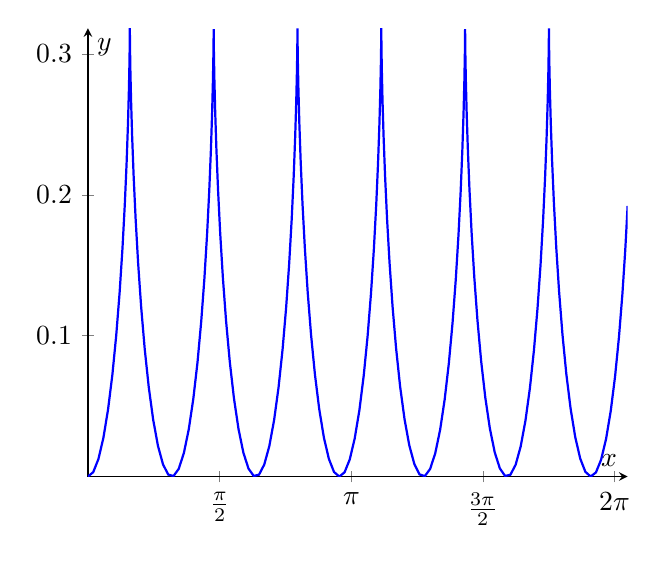
\begin{tikzpicture}
  \begin{axis}[
    trig format plots=rad,
    axis lines=middle,
    xlabel={$x$},
    ylabel={$y$},
    domain=0:6.28318,
    samples=200,
    xtick={0,1.5708,3.14159,4.71239,6.28318},
    xticklabels={$0$, $\frac{\pi}{2}$, $\pi$, $\frac{3\pi}{2}$, $2\pi$}
  ]
    % Gerstner wave (free surface)
    \addplot[
      blue,
      thick,
      variable=\t,
      parametric
    ] (
      { \t + (1/(2*pi)) * sin(2*pi*\t) },
      { (1/(2*pi)) * (1 - cos(2*pi*\t)) }
    );
  \end{axis}
\end{tikzpicture}
\caption{Γραφική παράσταση κύματος Gerstner (τροχοειδές κύμα) για μήκος κύματος $\lambda = 1$.}
\label{fig:gerstner}
\end{figure}

Κάθε σημείο της επιφάνειας δίνεται παραμετρικά:

\[x(u, t) = u - \frac{A \cdot k}{|k|} \sin(k u - \omega t + \varphi)\]

\[y(u, t) = A \cos(k u - \omega t + \varphi)\]

όπου \(u\) είναι η αρχική οριζόντια θέση κάθε σημείου.

\textbf{Παράμετροι:}

\begin{itemize}
\tightlist
\item
  \textbf{\(A\) (Πλάτος):} Ακτίνα της κυκλικής τροχιάς
\item
  \textbf{\(k\) (Κυματαριθμός):} \(k = \frac{2\pi}{\lambda}\)
\item
  \textbf{\(\omega\) (Γωνιακή συχνότητα):} \(\omega = \sqrt{g \cdot k}\)
  (σχέση διασποράς)
\item
  \textbf{\(\varphi\) (Αρχική φάση):} Οριζόντια μετατόπιση
\end{itemize}

\begin{quote}
Η σχέση \(\omega = \sqrt{gk}\) προκύπτει από τη θεωρία επιφανειακών
κυμάτων βαρύτητας σε βαθύ νερό.
\end{quote}

\subsection{Άθροισμα
συχνοτήτων}\label{ux3acux3b8ux3c1ux3bfux3b9ux3c3ux3bcux3b1-ux3c3ux3c5ux3c7ux3bdux3bfux3c4ux3aeux3c4ux3c9ux3bd}

Διαδραστικά προστίθενται συνιστώσες με διαφορετικές συχνότητες και
πλάτη. Οι μαθητές βλέπουν ότι το «σύνθετο» σήμα δεν είναι τίποτα
περισσότερο από υπέρθεση απλών κυμάτων.

\section{Ήχος}\label{ux3aeux3c7ux3bfux3c2}

Μέχρι τώρα μιλήσαμε για κύματα στο νερό. Αλλά η ίδια μαθηματική δομή
επανεμφανίζεται σε έναν άλλο, πιο οικείο τομέα --- τον ήχο. Το αυτί
κάνει φυσικά αυτό που ο Fourier κάνει αλγεβρικά.

\subsection{Το παράδειγμα του
ήχου}\label{ux3c4ux3bf-ux3c0ux3b1ux3c1ux3acux3b4ux3b5ux3b9ux3b3ux3bcux3b1-ux3c4ux3bfux3c5-ux3aeux3c7ux3bfux3c5}

Ο ήχος χρησιμοποιείται ως αναλογία: όπως το νερό είναι υπέρθεση
κυματικών συνιστωσών, έτσι και το ακουστικό σήμα αναλύεται σε απλά
ημίτονα. Συνδέεται η μαθηματική μορφή με την φυσική εικόνα πυκνώσεων και
αραιώσεων.

\subsection{Παράδειγμα ήχου
τάξης}\label{ux3c0ux3b1ux3c1ux3acux3b4ux3b5ux3b9ux3b3ux3bcux3b1-ux3aeux3c7ux3bfux3c5-ux3c4ux3acux3beux3b7ux3c2}

Οι συμμετέχοντες τροφοδοτούν παραμέτρους (συχνότητα/πλάτος) και
δημιουργούν συλλογικά σύνθετο σήμα. Η διαφάνεια μετατρέπει την ανάλυση
Fourier σε βιωματική ομαδική δραστηριότητα.

\subsection{Από σύνθετο ήχο σε 3
καθαρούς}\label{ux3b1ux3c0ux3cc-ux3c3ux3cdux3bdux3b8ux3b5ux3c4ux3bf-ux3aeux3c7ux3bf-ux3c3ux3b5-3-ux3baux3b1ux3b8ux3b1ux3c1ux3bfux3cdux3c2}

Γίνεται η αντίστροφη ανάγνωση: από ένα ενιαίο σύνθετο κύμα προς τις
βασικές συνιστώσες του. Έτσι σταθεροποιείται διαισθητικά η έννοια
«σύνθεση και ανάλυση είναι δύο όψεις του ίδιου μηχανισμού».

\section{Taylor}\label{taylor}

Για τους υπολογιστές, συναρτήσεις όπως οι \(\sin x\), \(\cos x\) των
ηχητικών κυμάτων είναι υπολογιστικά δαπανηρές. Τα πολυώνυμα, που
βασίζονται σε προσθέσεις και πολλαπλασιασμούς, είναι ευκολότερα
διαχειρίσιμα. Μια συνάρτηση γύρω από ένα σημείο \(x_0\) μπορεί να
προσεγγιστεί με ένα πολυώνυμο Taylor:

\[
f(x) = a_0 + a_1(x - x_0)^1 + a_2(x - x_0)^2 + a_3(x - x_0)^3 + \dots + a_n(x - x_0)^n
\]

Με παραγώγιση της \(f(x)\), προκύπτουν οι αντίστοιχοι συντελεστές
\(a_k\): \(a_0 = f(x_0)\), \(a_1 = f'(x_0)\),
\(a_2 = \dfrac{1}{2}\,f''(x_0)\), \ldots,
\(a_n = \frac{1}{n!}\,f^{(n)}(x_0)\). Αν το σημείο \(x_0\) είναι το
μηδέν, η σειρά ονομάζεται Maclaurin. Αν το ανάπτυγμα είναι άπειρο τότε
πρόκειται για σειρά Taylor \[
f(x) = \sum_{n=0}^{\infty} \frac{f^{(n)}(x_0)}{n!} (x - x_0)^n
\] Θα πρέπει η \(f\) να είναι ομαλή στο \(x_0\), δηλαδή να υπάρχουν
παράγωγοι κάθε τάξης \(f^{(n)}(x_0)\) για κάθε \(n \in \mathbb{N}\).

Το ανάπτυγμα Taylor (άπειρο) \textbf{δεν συγκλίνει πάντοτε} στην
\(f(x)\), ακόμα κι αν η \(f\) είναι ομαλή.\\
Χρειάζεται το υπόλοιπο \(R_N(x) \to 0\) καθώς \(N \to \infty\).

Για παράδειγμα:

\begin{itemize}
\tightlist
\item
  \textbf{Αναλυτικές συναρτήσεις} (π.χ.
  \(e^x, \sin x, \cos x, \ln(1+x)\) στο κατάλληλο διάστημα): η σειρά
  συγκλίνει στην \(f\) σε μία περιοχή γύρω από το \(x_0\) (ακτίνα
  σύγκλισης).
\item
  Μη αναλυτικές ομαλές συναρτήσεις (π.χ. \(e^{-1/x^2}\) για \(x \neq 0\)
  και \(0\) στο \(0\)): όλες οι παράγωγοι στο \(0\) είναι μηδέν, οπότε
  το ανάπτυγμα Taylor είναι μηδενικό, αλλά η συνάρτηση δεν είναι μηδέν
  για \(x \neq 0\). Εδώ η σειρά \textbf{δεν συγκλίνει} στην \(f\).
\end{itemize}

Για \textbf{οποιαδήποτε} \(N\) φορές παραγωγίσιμη συνάρτηση, μπορούμε να
γράψουμε:

\[
f(x) = \underbrace{\sum_{n=0}^{N} \frac{f^{(n)}(x_0)}{n!} (x-x_0)^n}_{\text{πολυώνυμο Taylor}} + R_N(x)
\]

όπου \(R_N(x)\) το υπόλοιπο (τύπος Lagrange, Cauchy, κ.λπ.).\\
Το πολυώνυμο υπάρχει πάντα, αλλά προσεγγίζει την \(f\) μόνο κοντά στο
\(x_0\) και με σφάλμα που εξαρτάται από την \((N+1)\)-η παράγωγο.

\begin{itemize}
\tightlist
\item
  \textbf{Πεπερασμένο ανάπτυγμα} (πολυώνυμο): αρκεί η \(f\) να είναι
  \(N\) φορές παραγωγίσιμη στο \(x_0\).
\item
  \textbf{Άπειρη σειρά Taylor} που συγκλίνει στην \(f\): απαιτείται η
  \(f\) να είναι \textbf{αναλυτική} στο \(x_0\) (δηλαδή η σειρά
  συγκλίνει και ταυτίζεται με την \(f\) σε μια περιοχή).
\end{itemize}

Στην πράξη, όλες οι συναρτήσεις που συναντάμε σε ηχητικά σήματα
(ημίτονα, εκθετικές) είναι αναλυτικές, άρα το ανάπτυγμα Taylor ισχύει
και συγκλίνει.

\subsection{\texorpdfstring{\(e^{x/2}\cos(x)\)}{e\^{}\{x/2\}\textbackslash cos(x)}}\label{ex2cosx}

Η καλύτερη γραμμική προσέγγιση μιας συνάρτησης σε ένα σημείο είναι
εκείνη για την οποία η τιμή και η παράγωγος της προσέγγισης συμπίπτουν
με την τιμή και την παράγωγο της συνάρτησης στο σημείο αυτό.

Για τη συνάρτηση \(f(x) = e^{x/2} \cos(x)\), στο σημείο \(x = 0\)
υπολογίζουμε
\(f'(x) = \frac{1}{2} e^{x/2} \cos(x) - e^{x/2} \sin(x) = e^{x/2} \left( \frac{1}{2} \cos(x) - \sin(x) \right)\),
άρα:

\begin{itemize}
\item
  \(f(0) = e^{0} \cos(0) = 1 \cdot 1 = 1\),
\item
  \(f'(0) = e^{0} \left( \frac{1}{2} \cdot 1 - 0 \right) = \frac{1}{2}\).
\end{itemize}

Επομένως, η γραμμική προσέγγιση (πολυώνυμο Taylor πρώτου βαθμού) είναι:

\[
\boxed{T_1(x) = f(0) + f'(0) \, x = 1 + \frac{x}{2}}.
\]

\begin{figure}[htbp]
\centering
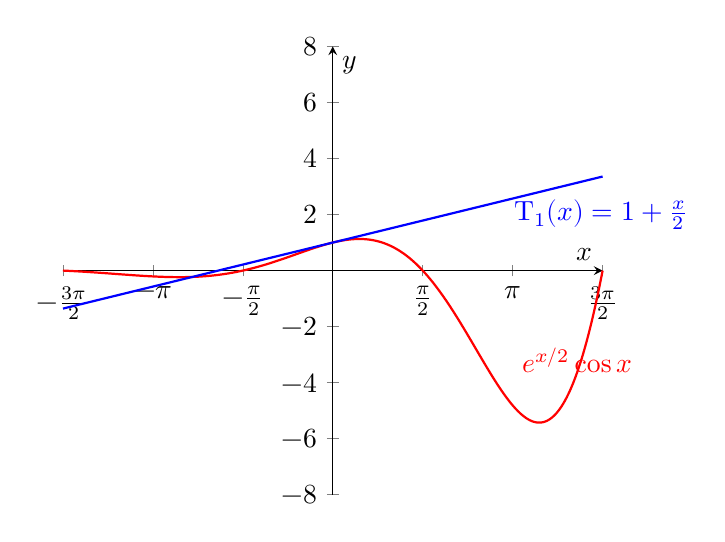
\begin{tikzpicture}
  \begin{axis}[
    trig format plots=rad,
    axis lines=middle,
    xlabel={$x$},
    ylabel={$y$},
    domain=-1.5*pi:1.5*pi,
    samples=300,
    ymin=-8,
    ymax=8,
    clip=false,
    xtick={-6.28318, -4.71239, -3.14159, -1.5708, 0, 1.5708, 3.14159, 4.71239, 6.28318},
    xticklabels={$-2\pi$, $-\frac{3\pi}{2}$, $-\pi$, $-\frac{\pi}{2}$, $0$, $\frac{\pi}{2}$, $\pi$, $\frac{3\pi}{2}$, $2\pi$},
    ytick={-8,-6,-4,-2,0,2,4,6,8},
  ]
    \addplot[red, thick] {exp(x/2)*cos(x)};
    \addplot[blue, thick] {1 + 0.5*x};
    
    % Τοποθέτηση ετικετών
    \node[red, anchor=west] at (axis cs:3.14, {exp(3.14/2)*cos(3.14)-8}) {$e^{x/2}\cos x$};
    \node[blue, anchor=west] at (axis cs:3., {1 + 0.5*3.-0.5}) {$Τ_1(x)=1+\frac{x}{2}$};
  \end{axis}
\end{tikzpicture}
\caption{Σύγκριση $e^{x/2}\cos x$ με γραμμική προσέγγιση $1+x/2$}
\label{fig:expcoslinear}
\end{figure}

Για τη δεύτερη παράγωγο: \[
f''(x) = \frac{d}{dx} \left[ e^{x/2} \left( \frac{1}{2}\cos x - \sin x \right) \right] 
= \dots 
= e^{x/2} \left( -\frac{3}{4}\cos x - \sin x \right),
\]

οπότε στο \(x=0\):

\[
f''(0) = e^{0} \left( -\frac{3}{4} \cdot 1 - 0 \right) = -\frac{3}{4}.
\] Έτσι, η τετραγωνική προσέγγιση (πολυώνυμο Taylor δεύτερου βαθμού)
είναι:

\[
\boxed{T_2(x) = f(0) + f'(0)\,x + \frac{f''(0)}{2}\,x^2 = 1 + \frac{x}{2} - \frac{3}{8}x^2}.
\]

Σημειώνεται ότι, ενώ η δεύτερη παράγωγος της συνάρτησης στο \(0\) είναι
\(-\frac{3}{4}\), πρέπει να ληφθεί υπόψη ότι, για έναν όρο \(a x^2\) στο
πολυώνυμο, ισχύει \[
\frac{d}{dx}(a x^2)=2ax \quad \text{και} \quad \frac{d^2}{dx^2}(a x^2)=2a.
\] Άρα, αφού \(P''(0)=2a=-\frac{3}{4}\), προκύπτει \(a=-\frac{3}{8}\).

Αν η διαδικασία συνεχιστεί, είναι προφανές ότι κάθε πολυώνυμο
μεγαλύτερου βαθμού ---και, αντίστοιχα, οι παράγωγοι μεγαλύτερης τάξης---
θα ενσωματώνει στο πολυώνυμο περισσότερη πληροφορία, οδηγώντας σε ολοένα
και καλύτερη προσέγγιση. Η αναπαράσταση μιας συνάρτησης ως άπειρο
άθροισμα πολυωνυμικών όρων ονομάζεται Σειρά Taylor.

\begin{figure}[htbp]
\centering
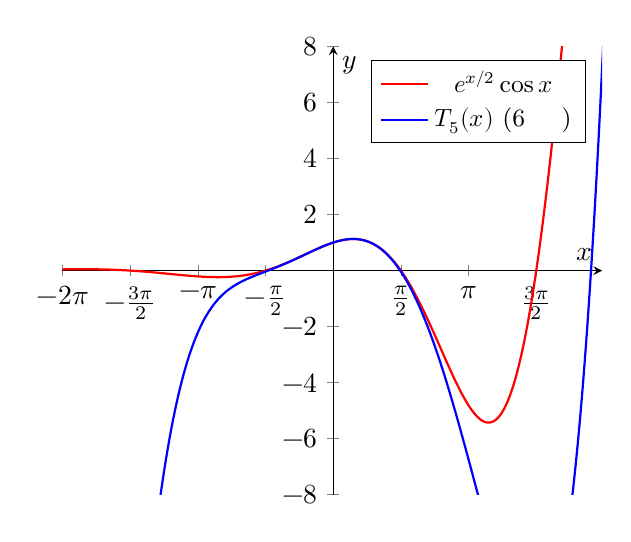
\begin{tikzpicture}
  \begin{axis}[
    trig format plots=rad,
    axis lines=middle,
    xlabel={$x$},
    ylabel={$y$},
    domain=-2*pi:2*pi,
    samples=300,
    ymin=-8,
    ymax=8,
    xtick={-6.28318, -4.71239, -3.14159, -1.5708, 0, 1.5708, 3.14159, 4.71239, 6.28318},
    xticklabels={$-2\pi$, $-\frac{3\pi}{2}$, $-\pi$, $-\frac{\pi}{2}$, $0$, $\frac{\pi}{2}$, $\pi$, $\frac{3\pi}{2}$, $2\pi$},
    ytick={-8,-6,-4,-2,0,2,4,6,8},
    legend pos=north east,
    legend style={font=\small}
  ]
    \addplot[red, thick] {exp(x/2)*cos(x)};
    \addlegendentry{$e^{x/2}\cos x$}
    
    \addplot[blue, thick] {1 + 0.5*x - 0.375*x^2 - 0.2291666667*x^3 - 0.0182291667*x^4 + 0.0106770833*x^5};
    \addlegendentry{$T_5(x)$ (6 όροι)}
  \end{axis}
\end{tikzpicture}
\caption{Σύγκριση $e^{x/2}\cos x$ με το πολυώνυμο Taylor 5ου βαθμού.}
\label{fig:expcostaylor}
\par
\end{figure}

Ο γενικός τύπος της σειράς γύρω από το \(0\) (γνωστός και ως ανάπτυγμα
Maclaurin) είναι η έκφραση:

\[f(x) = f(0) + \frac{f'(0)}{1!}x + \frac{f''(0)}{2!}x^2 + \frac{f'''(0)}{3!}x^3 + \dots\]

όπου κάθε επόμενος όρος προστίθεται για να ``διορθώσει'' την προσέγγιση,
χρησιμοποιώντας ολοένα και υψηλότερες παραγώγους.

\subsection{\texorpdfstring{\(\cos(x)\)}{\textbackslash cos(x)}}\label{cosx}

Η συνάρτηση \(\cos(x)\) είναι άρτια, οπότε στο ανάπτυγμα Maclaurin
(σειρά Taylor γύρω από το \(0\)) εμφανίζονται μόνο άρτιες δυνάμεις του
\(x\). Υπολογίζοντας τις παραγώγους:

\[
\begin{aligned}
f(0) &= \cos(0) = 1, \\
f'(0) &= -\sin(0) = 0, \\
f''(0) &= -\cos(0) = -1, \\
f'''(0) &= \sin(0) = 0, \\
f^{(4)}(0) &= \cos(0) = 1, \quad \text{κ.ο.κ.}
\end{aligned}
\]

Αντικαθιστώντας στον τύπο
\(f(x)=\sum_{n=0}^{\infty} \frac{f^{(n)}(0)}{n!}x^n\), προκύπτει:

\[
\cos(x) = 1 - \frac{x^2}{2!} + \frac{x^4}{4!} - \frac{x^6}{6!} + \cdots = \sum_{n=0}^{\infty} (-1)^n \frac{x^{2n}}{(2n)!}
\]

Για παράδειγμα, κοντά στο \(0\):

\begin{itemize}
\item
  Το πολυώνυμο \(1\) δίνει \(\cos(x)\approx 1\).
\item
  Το πολυώνυμο \(1 - \frac{x^2}{2}\) διορθώνει την προσέγγιση για μικρά
  \(x\).
\item
  Προσθέτοντας τον όρο \(\frac{x^4}{24}\) γίνεται ακόμη καλύτερη
  προσέγγιση.
\end{itemize}

\begin{figure}[htbp]
\centering
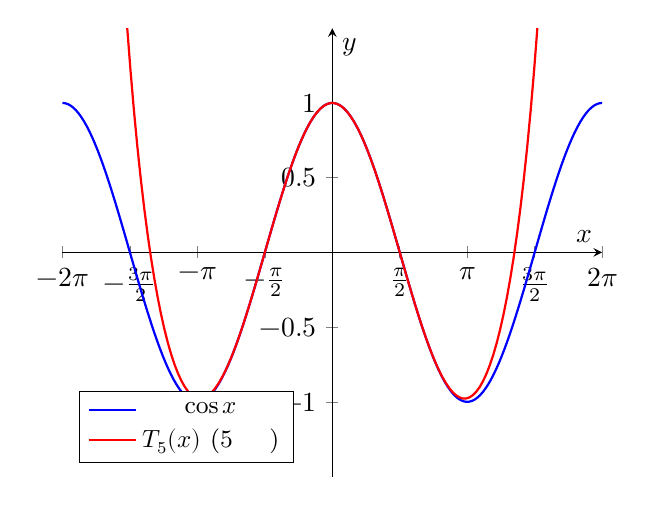
\begin{tikzpicture}
  \begin{axis}[
    trig format plots=rad,
    axis lines=middle,
    xlabel={$x$},
    ylabel={$y$},
    domain=-2*pi:2*pi,
    samples=200,
    ymin=-1.5, ymax=1.5,
    xtick={-6.28318, -4.71239, -3.14159, -1.5708, 0, 1.5708, 3.14159, 4.71239, 6.28318},
    xticklabels={$-2\pi$, $-\frac{3\pi}{2}$, $-\pi$, $-\frac{\pi}{2}$, $0$, $\frac{\pi}{2}$, $\pi$, $\frac{3\pi}{2}$, $2\pi$},
    ytick={-1, -0.5, 0, 0.5, 1},
    legend pos=south west,
    legend style={font=\small}
  ]
    \addplot[blue, thick] {cos(x)};
    \addlegendentry{$\cos x$}
    
    \addplot[red, thick, domain=-2.5*pi:2.5*pi] {1 - x^2/2 + x^4/24 - x^6/720 + x^8/40320};
    \addlegendentry{$T_5(x)$ (5 όροι)}
  \end{axis}
\end{tikzpicture}
\caption{Σύγκριση $\cos x$ με το πολυώνυμο Taylor 5 όρων (έως $x^8$).}
\label{fig:costaylor5}
\par
\end{figure}

\subsection{\texorpdfstring{\(\sin(x)\)}{\textbackslash sin(x)}}\label{sinx}

Αντίστοιχα, το \(\sin(x)\) είναι περιττή συνάρτηση, οπότε το ανάπτυγμα
περιέχει μόνο περιττές δυνάμεις. Οι παράγωγοι στο \(0\) δίνουν:

\[
\sin(0)=0,\; \cos(0)=1,\; -\sin(0)=0,\; -\cos(0)=-1,\; \sin(0)=0,\; \dots
\]

Έτσι:

\[
\sin(x) = x - \frac{x^3}{3!} + \frac{x^5}{5!} - \frac{x^7}{7!} + \cdots = \sum_{n=0}^{\infty} (-1)^n \frac{x^{2n+1}}{(2n+1)!}
\]

Παρατηρούμε ότι η σειρά του \(\cos(x)\) είναι ακριβώς η παράγωγος όρο
προς όρο της σειράς του \(\sin(x)\), κάτι που συμφωνεί με τη γνωστή
παραγώγιση \((\sin x)' = \cos x\).

\begin{figure}[htbp]
\centering
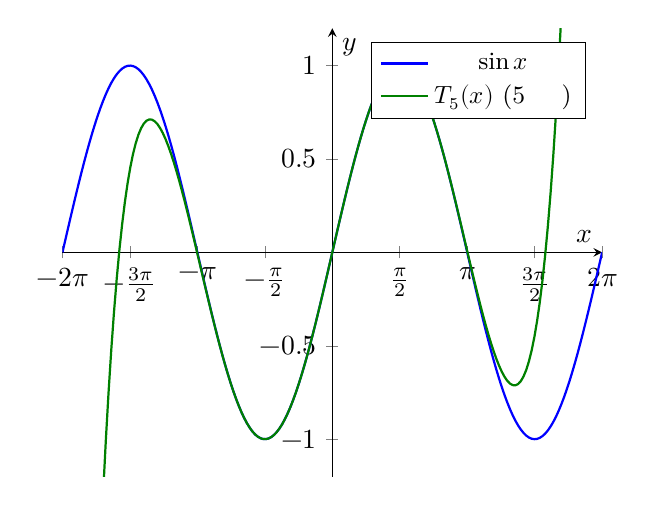
\begin{tikzpicture}
  \begin{axis}[
    trig format plots=rad,
    axis lines=middle,
    xlabel={$x$},
    ylabel={$y$},
    domain=-4*pi:4*pi,
    samples=200,
    ymin=-1.2,
    ymax=1.2,
    xtick={-6.28318, -4.71239, -3.14159, -1.5708, 0, 1.5708, 3.14159, 4.71239, 6.28318},
    xticklabels={$-2\pi$, $-\frac{3\pi}{2}$, $-\pi$, $-\frac{\pi}{2}$, $0$, $\frac{\pi}{2}$, $\pi$, $\frac{3\pi}{2}$, $2\pi$},
    ytick={-1, -0.5, 0, 0.5, 1},
    legend pos=north east,
    legend style={font=\small}
  ]
    
    % Sinc
    \addplot[blue, thick, domain=-2*pi:2*pi] {sin(x)};
    \addlegendentry{$\sin x$}
    
     % Taylor 5 όρων (έως x^9)
    \addplot[green!50!black, thick, domain=-2*pi:2*pi] {x - x^3/6 + x^5/120 - x^7/5040 + x^9/362880};
    \addlegendentry{$T_5(x)$ (5 όροι)}
    
     
  \end{axis}
\end{tikzpicture}
\caption{Σύγκριση του $\sin x$ με πολυώνυμο Taylor 5 όρων.}
\label{fig:sintaylor}
\par
\end{figure}

\subsection{\texorpdfstring{\(e^x\)}{e\^{}x}}\label{ex}

Η εκθετική συνάρτηση \(e^x\) έχει την ιδιότητα να ισούται με κάθε της
παράγωγο: \((e^x)^{(n)} = e^x\). Επομένως, στο \(x=0\):

\[
f^{(n)}(0) = e^0 = 1 \quad \text{για κάθε } n.
\]

Ο τύπος Maclaurin δίνει:

\[
e^x = 1 + x + \frac{x^2}{2!} + \frac{x^3}{3!} + \frac{x^4}{4!} + \cdots = \sum_{n=0}^{\infty} \frac{x^n}{n!}
\] Αυτό είναι ίσως το σημαντικότερο ανάπτυγμα Taylor, καθώς αποτελεί τη
βάση για ορισμούς και πολλές εφαρμογές. Η σειρά συγκλίνει και πάλι για
κάθε \(x\), με ακτίνα σύγκλισης \(R=\infty\).

\begin{figure}[htbp]
\centering
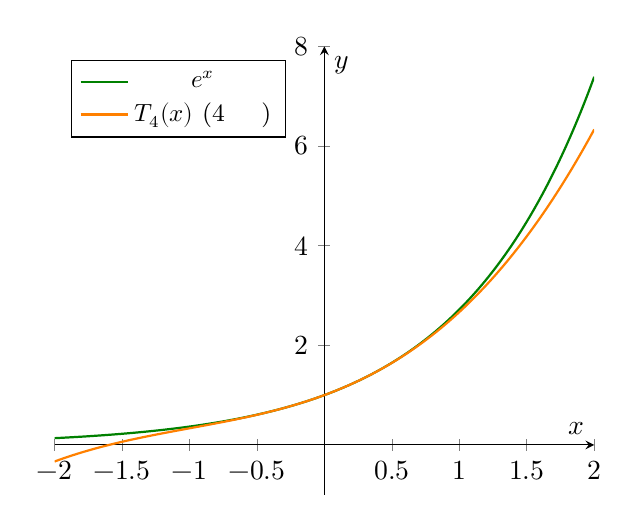
\begin{tikzpicture}
  \begin{axis}[
    axis lines=middle,
    xlabel={$x$},
    ylabel={$y$},
    domain=-2:2,
    samples=200,
    ymin=-1,
    ymax=8,
    xtick={-2,-1.5,-1,-0.5,0,0.5,1,1.5,2},
    ytick={0,2,4,6,8},
    legend pos=north west,
    legend style={font=\small}
  ]
    \addplot[green!50!black, thick] {exp(x)};
    \addlegendentry{$e^x$}
    
    \addplot[orange, thick] {1 + x + x^2/2 + x^3/6};
    \addlegendentry{$T_4(x)$ (4 όροι)}
  \end{axis}
\end{tikzpicture}
\caption{Σύγκριση $e^x$ με το πολυώνυμο Taylor 5ου βαθμού (6 όροι).}
\label{fig:exptaylor}
\par
\end{figure}

\section{Euler}\label{euler}

Τα αναπτύγματα του \(\sin x\) \(\cos x\) και \(e^x\) μοιάζουν
ανεξάρτητα. Αλλά αν αντικαταστήσουμε το \(x\) με \(i^x\) στο ανάπτυγμα
του \(e^x\) και οι τρεις συναρτήσεις αποκαλύπτονται ως μία.

\begin{figure}[htbp]
\centering
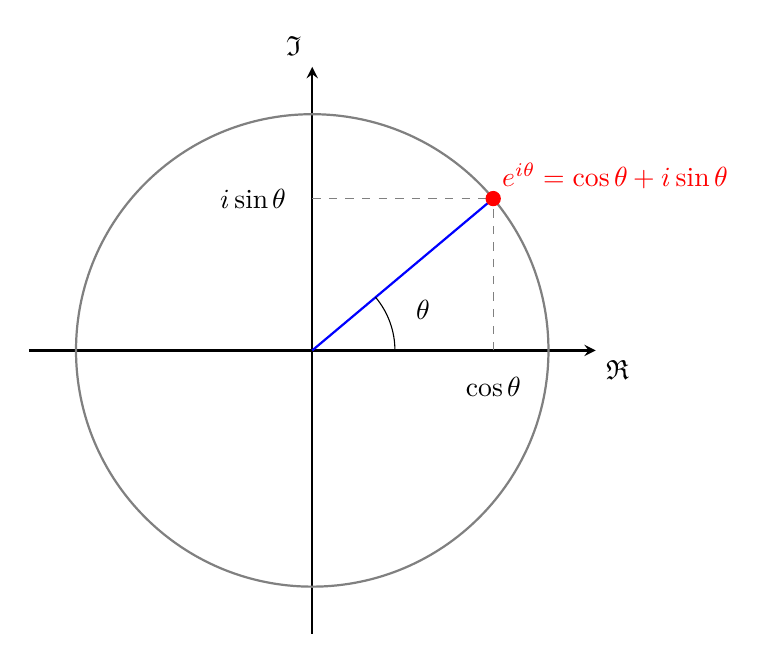
\begin{tikzpicture}[scale=3,>=stealth]
  % Άξονες
  \draw[->,thick] (-1.2,0) -- (1.2,0) node[below right] {$\Re$};
  \draw[->,thick] (0,-1.2) -- (0,1.2) node[above left] {$\Im$};
  
  % Μοναδιαίος κύκλος
  \draw[gray, thick] (0,0) circle (1);
  
  % Γωνία θ (π.χ. 40°)
  \def\angle{40}
  
  % Διακεκομμένες προβολές
  \draw[dashed, gray] ({cos(\angle)},0) -- ({cos(\angle)},{sin(\angle)});
  \draw[dashed, gray] (0,{sin(\angle)}) -- ({cos(\angle)},{sin(\angle)});
  
  % Διάνυσμα από την αρχή
  \draw[blue, thick] (0,0) -- ({cos(\angle)},{sin(\angle)});
  
  % Σημείο e^{iθ}
  \filldraw[red] ({cos(\angle)},{sin(\angle)}) circle (0.03) 
    node[above right] {$e^{i\theta} = \cos\theta + i\sin\theta$};
  
  % Τόξο για τη γωνία
  \draw (0.35,0) arc (0:\angle:0.35);
  \node at ({\angle/2}:0.5) {$\theta$};
  
  % Ετικέτες στους άξονες
  \node at ({cos(\angle)}, -0.07) [below] {$\cos\theta$};
  \node at (-0.07, {sin(\angle)}) [left] {$i\sin\theta$};
\end{tikzpicture}
\caption{Μιγαδικό επίπεδο: η γραφική αναπαράσταση του τύπου του Euler.}
\label{fig:euler}
\par   % αποφυγή σφάλματος \prevdepth
\end{figure}

Γνωρίζοντας τα αναπτύγματα των \(\sin x\), \(\cos x\) και \(e^x\),
μπορούμε να ανακαλύψουμε τη σχέση \textbf{Euler}. Αν αντικαταστήσουμε
\(x\) με \(ix\) στο ανάπτυγμα της \(e^x\) (όπου \(i^2=-1\)) και
ομαδοποιήσουμε πραγματικούς και φανταστικούς όρους, θα προκύψει
\(e^{ix} = \cos x + i\sin x\) που συνδέει τις τρεις αυτές θεμελιώδεις
συναρτήσεις.

Ξεκινάμε από το ανάπτυγμα της εκθετικής συνάρτησης:

\[
e^{x} = \sum_{n=0}^{\infty} \frac{x^n}{n!} = 1 + x + \frac{x^2}{2!} + \frac{x^3}{3!} + \frac{x^4}{4!} + \frac{x^5}{5!} + \frac{x^6}{6!} + \cdots
\]

Αντικαθιστούμε το \(x\) με \(ix\), όπου \(i\) είναι η φανταστική μονάδα
(\(i^2 = -1\), \(i^3 = -i\), \(i^4 = 1\), \(i^5 = i\), κ.ο.κ.):

\[
e^{ix} = \sum_{n=0}^{\infty} \frac{(ix)^n}{n!} = 1 + ix + \frac{(ix)^2}{2!} + \frac{(ix)^3}{3!} + \frac{(ix)^4}{4!} + \frac{(ix)^5}{5!} + \frac{(ix)^6}{6!} + \cdots
\]

Υπολογίζουμε τις δυνάμεις του \(i\):

\begin{itemize}
\tightlist
\item
  \((ix)^0 = 1\)
\item
  \((ix)^1 = i x\)
\item
  \((ix)^2 = i^2 x^2 = -x^2\)
\item
  \((ix)^3 = i^3 x^3 = -i x^3\)
\item
  \((ix)^4 = i^4 x^4 = x^4\)
\item
  \((ix)^5 = i^5 x^5 = i x^5\)
\item
  \((ix)^6 = i^6 x^6 = -x^6\)
\item
  \((ix)^7 = i^7 x^7 = -i x^7\)
\item
  κ.ο.κ.
\end{itemize}

Αντικαθιστώντας:

\[
e^{ix} = 1 + ix + \frac{-x^2}{2!} + \frac{-i x^3}{3!} + \frac{x^4}{4!} + \frac{i x^5}{5!} + \frac{-x^6}{6!} + \frac{-i x^7}{7!} + \cdots
\]

Ομαδοποιούμε τώρα τους \textbf{πραγματικούς} όρους (αυτούς που δεν
πολλαπλασιάζονται με \(i\)) και τους \textbf{φανταστικούς} όρους (αυτούς
που περιέχουν \(i\)).

\textbf{Πραγματικοί όροι}: προέρχονται από άρτιες δυνάμεις
\(n = 0,2,4,6,\dots\) (γιατί οι περιττές δίνουν παράγοντα \(i\)).
Συγκεκριμένα:

\[
n=0:\; 1,\quad n=2:\; -\frac{x^2}{2!},\quad n=4:\; \frac{x^4}{4!},\quad n=6:\; -\frac{x^6}{6!},\quad \dots
\]

Δηλαδή:

\[
\operatorname{Re}(e^{ix}) = 1 - \frac{x^2}{2!} + \frac{x^4}{4!} - \frac{x^6}{6!} + \cdots
\]

Το άθροισμα αυτό είναι ακριβώς το ανάπτυγμα Taylor του \(\cos x\) (βλ.
§4.2):

\[
\cos x = \sum_{n=0}^{\infty} (-1)^n \frac{x^{2n}}{(2n)!} = 1 - \frac{x^2}{2!} + \frac{x^4}{4!} - \frac{x^6}{6!} + \cdots
\]

\textbf{Φανταστικοί όροι}: προέρχονται από περιττές δυνάμεις
\(n = 1,3,5,7,\dots\) και περιέχουν τον παράγοντα \(i\). Γράφουμε:

\[
n=1:\; i x,\quad n=3:\; -\frac{i x^3}{3!},\quad n=5:\; \frac{i x^5}{5!},\quad n=7:\; -\frac{i x^7}{7!},\quad \dots
\]

Βγάζοντας κοινό παράγοντα \(i\):

\[
\operatorname{Im}(e^{ix}) = i\left( x - \frac{x^3}{3!} + \frac{x^5}{5!} - \frac{x^7}{7!} + \cdots \right)
\]

Η παρένθεση είναι το ανάπτυγμα Taylor του \(\sin x\) (βλ. §4.3):

\[
\sin x = \sum_{n=0}^{\infty} (-1)^n \frac{x^{2n+1}}{(2n+1)!} = x - \frac{x^3}{3!} + \frac{x^5}{5!} - \frac{x^7}{7!} + \cdots
\]

Επομένως:

\[
e^{ix} = \underbrace{\left(1 - \frac{x^2}{2!} + \frac{x^4}{4!} - \cdots \right)}_{\cos x} \;+\; i\underbrace{\left(x - \frac{x^3}{3!} + \frac{x^5}{5!} - \cdots \right)}_{\sin x}
\]

Τελικά:

\[
\boxed{e^{ix} = \cos x + i\sin x}
\]

Αυτή η ταυτότητα συνδέει την εκθετική με τις τριγωνομετρικές συναρτήσεις
στο μιγαδικό πεδίο και αποτελεί το θεμέλιο για τις σειρές Fourier, την
ανάλυση κυματομορφών και άλλες εφαρμογές στη φυσική και τη μηχανική.

\subsection{Ο i ως περιστροφή και
ανάπτυγμα}\label{ux3bf-i-ux3c9ux3c2-ux3c0ux3b5ux3c1ux3b9ux3c3ux3c4ux3c1ux3bfux3c6ux3ae-ux3baux3b1ux3b9-ux3b1ux3bdux3acux3c0ux3c4ux3c5ux3b3ux3bcux3b1}

Ο πολλαπλασιασμός με \(i\) ερμηνεύεται ως περιστροφή κατά \(90^\circ\).
Από εκεί προκύπτει φυσικά η σύνδεση με τη σχέση του Euler και η μετάβαση
σε κυκλική αναπαράσταση ταλαντώσεων.

\section{Σειρές Fourier}\label{ux3c3ux3b5ux3b9ux3c1ux3adux3c2-fourier}

Ο Fourier (1768--1830), εμπνευσμένος από το πρακτικό πρόβλημα της
θερμικής μόνωσης κτιρίων που τον απασχόλησε κατά τη θητεία του ως
σύμβουλος του Ναπολέοντα στην Αίγυπτο, ανέπτυξε μια πρωτοποριακή
μαθηματική θεωρία για τη διάδοση της θερμότητας, απορρίπτοντας τις
θεωρίες της εποχής του και στηριζόμενος αποκλειστικά στις εξισώσεις. Το
1807 παρουσίασε στην Ακαδημία Επιστημών του Παρισιού την εξίσωση
θερμότητας και, για να τη λύσει, εφηύρε τις σειρές Fourier. Την ανάλυση
δηλαδή οποιασδήποτε ομαλής συνάρτησης ως άθροισμα απείρων ημιτόνων και
συνημιτόνων, μια προσέγγιση ανάλογη με το ανάπτυγμα Taylor, όπου η
συνάρτηση εκφράζεται ως άθροισμα πολυωνυμικών όρων. Αν και αρχικά
αμφισβητήθηκε για έλλειψη μαθηματικής αυστηρότητας, το έργο του
δημοσιεύτηκε πλήρως δεκαπέντε χρόνια αργότερα στο Théorie analytique de
la chaleur (1822).

\subsection{Διάχυση θερμότητας με
ημίτονο}\label{ux3b4ux3b9ux3acux3c7ux3c5ux3c3ux3b7-ux3b8ux3b5ux3c1ux3bcux3ccux3c4ux3b7ux3c4ux3b1ux3c2-ux3bcux3b5-ux3b7ux3bcux3afux3c4ux3bfux3bdux3bf}

Αν θερμάνουμε ένα μικρό τμήμα μιας μονωμένης μεταλλικής ράβδου και το
αφήσουμε για αρκετή ώρα, η καθημερινή μας εμπειρία από τη διάχυση της
θερμότητας μάς επιτρέπει να προβλέψουμε ότι η θερμοκρασία θα εξομαλυνθεί
μέχρι να γίνει ομοιόμορφη. Σε συνθήκες τέλειας μόνωσης, η θερμότητα θα
παραμείνει στο μέταλλο για πάντα. ια τρία γειτονικά σημεία
\(T_1, T_2, T_3\):

\[\frac{dT_2}{dt} = \alpha \left(\frac{T_1 + T_3}{2} - T_2\right)\]

Αυτό είναι η \textbf{διαφορά των διαφορών} --- δηλαδή η δεύτερη
παράγωγος ως προς τον χώρο.

Στο συνεχές όριο (άπειρα σημεία) γίνεται:

\[\frac{\partial T}{\partial t} = \alpha \frac{\partial^2 T}{\partial x^2}\]

Διαβάζεται: \emph{«ο ρυθμός αλλαγής θερμοκρασίας στον χρόνο εξαρτάται
από την καμπυλότητα της κατανομής στον χώρο»}.

\begin{quote}
Όπου η κατανομή \textbf{κυρτώνει προς τα πάνω}, η θερμοκρασία
\textbf{ανεβαίνει}.\\
Όπου \textbf{κυρτώνει προς τα κάτω}, \textbf{κατεβαίνει}.\\
Οι ανωμαλίες εξομαλύνονται.
\end{quote}

\begin{center}\rule{0.5\linewidth}{0.5pt}\end{center}

\subsection{Ο Fourier μπροστά στο
πρόβλημα}\label{ux3bf-fourier-ux3bcux3c0ux3c1ux3bfux3c3ux3c4ux3ac-ux3c3ux3c4ux3bf-ux3c0ux3c1ux3ccux3b2ux3bbux3b7ux3bcux3b1}

Ο Fourier ρώτησε: μπορώ να γράψω μια \textbf{αυθαίρετη} αρχική κατανομή
\(T(x, 0)\) ως άθροισμα ημιτόνων;

\[T(x, 0) = \sum_{n=1}^{\infty} a_n \sin(n\pi x)\]

Αν ναι, τότε κάθε αρμονική εξελίσσεται ανεξάρτητα:

\[T(x, t) = \sum_{n=1}^{\infty} a_n \, e^{-\alpha n^2 \pi^2 t} \sin(n\pi x)\]

Παρατήρησε τι συμβαίνει με τον χρόνο:

\begin{longtable}[]{@{}ll@{}}
\toprule\noalign{}
Αρμονική & Ρυθμός απόσβεσης \\
\midrule\noalign{}
\endhead
\bottomrule\noalign{}
\endlastfoot
\(n=1\) (χαμηλή) & αργά \\
\(n=5\) (μέση) & γρηγορότερα \\
\(n=20\) (υψηλή) & πολύ γρήγορα \\
\end{longtable}

\textbf{Οι υψηλές συχνότητες σβήνουν πρώτες.}\\
Γι' αυτό η ράβδος εξομαλύνεται με τον χρόνο.

\begin{center}\rule{0.5\linewidth}{0.5pt}\end{center}

\subsubsection{\texorpdfstring{Πώς βρίσκουμε τους συντελεστές
\(a_n\);}{Πώς βρίσκουμε τους συντελεστές a\_n;}}\label{ux3c0ux3ceux3c2-ux3b2ux3c1ux3afux3c3ux3baux3bfux3c5ux3bcux3b5-ux3c4ux3bfux3c5ux3c2-ux3c3ux3c5ux3bdux3c4ux3b5ux3bbux3b5ux3c3ux3c4ux3adux3c2-a_n}

\[a_n = 2\int_0^1 T(x,0)\,\sin(n\pi x)\,dx\]

Πολλαπλασιάζουμε την άγνωστη κατανομή με μια \textbf{γνωστή αρμονική}
και ολοκληρώνουμε.

\begin{itemize}
\tightlist
\item
  Αν «ταιριάζουν» → μεγάλο αποτέλεσμα
\item
  Αν δεν ταιριάζουν → μηδενίζεται
\end{itemize}

Αυτή η ιδέα δεν ανήκει μόνο στη θερμότητα.

Στην επόμενη ενότητα θα δούμε ότι η ίδια ακριβώς λογική --- πόσο από
κάθε συχνότητα κρύβεται μέσα σε ένα σήμα --- αποτελεί τον μετασχηματισμό
Fourier.

\subsection{Step function σε ράβδο 1
m}\label{step-function-ux3c3ux3b5-ux3c1ux3acux3b2ux3b4ux3bf-1-m}

Μια ασυνεχής αρχική συνθήκη αναπτύσσεται σε σειρά Fourier και
παρατηρείται η σταδιακή σύγκλιση με περισσότερους όρους. Η διαφάνεια
συνδέει μαθηματική ανάλυση με πραγματικό διάχυτο φαινόμενο.

\subsection{Σύνθεση
Fourier}\label{ux3c3ux3cdux3bdux3b8ux3b5ux3c3ux3b7-fourier}

Κάθε συνάρτηση μιας μεταβλητής είτε συνεχής είτε ασυνεχής, μπορεί να
επεκταθεί σε μια σειρά ημιτόνων πολλαπλασίων της μεταβλητής

\section{Μετασχηματισμός
Fourier}\label{ux3bcux3b5ux3c4ux3b1ux3c3ux3c7ux3b7ux3bcux3b1ux3c4ux3b9ux3c3ux3bcux3ccux3c2-fourier}

Η ράβδος και η εξίσωση θερμότητας δεν ήταν παρά η αφετηρία. Εκεί
γεννήθηκε η βασική ιδέα --- ότι μια περιοδική συνάρτηση μπορεί να
αναλυθεί σε άθροισμα ημιτόνων και συνημιτόνων --- αλλά η δύναμη της
μεθόδου δεν μπορούσε να μείνει κλεισμένη στα όρια ενός φυσικού
προβλήματος. Το επόμενο βήμα ήταν η γενίκευση: ο Μετασχηματισμός Fourier
απελευθερώνει το εργαλείο από την περιοδικότητα και το εφαρμόζει σε
οποιοδήποτε σήμα, οποιασδήποτε μορφής. Από την περιγραφή της θερμότητας
σε μια ράβδο, φτάνουμε σε ένα καθολικό μαθηματικό πρίσμα που διαλύει
κάθε σήμα στις συχνοτικές του συνιστώσες --- και αυτό ακριβώς το κάνει
σήμερα θεμελιώδες εργαλείο σε κάθε πεδίο της επιστήμης και της
τεχνολογίας. \#\# Από το σήμα στο φάσμα (Fourier Transform)

Ο τύπος του Euler που είδαμε στην ενότητα 5:

\[e^{i\theta} = \cos\theta + i\sin\theta\]

είναι η καρδιά του μετασχηματισμού. Με \(\theta = -\frac{2\pi kn}{N}\):

\[e^{-i\frac{2\pi kn}{N}} = \cos\!\left(\frac{2\pi kn}{N}\right) - i\sin\!\left(\frac{2\pi kn}{N}\right)\]

Άρα ο DFT γράφεται:

\[\begin{split}
X_k &= \sum_{n=0}^{N-1} x_n \cdot e^{-i\frac{2\pi kn}{N}} \\[6pt]
    &= \sum_{n=0}^{N-1} x_n \left[\cos\!\left(\frac{2\pi kn}{N}\right)
       - i\sin\!\left(\frac{2\pi kn}{N}\right)\right]
\end{split}\]

και άρα η πράξη που εκτελείται είναι ουσιαστικά:

\[\begin{split}
\operatorname{Re}(X_k) &= \sum_{n=0}^{N-1} x_n\cos\!\left(\frac{2\pi kn}{N}\right), \\
\operatorname{Im}(X_k) &= -\sum_{n=0}^{N-1} x_n\sin\!\left(\frac{2\pi kn}{N}\right).
\end{split}\]

\textbf{Τι σημαίνει αυτό γεωμετρικά:}

\begin{itemize}
\tightlist
\item
  Κάθε δείγμα \(x_n\) πολλαπλασιάζεται με ένα σημείο στον μοναδιαίο
  κύκλο γωνίας \(-\frac{2\pi kn}{N}\)
\item
  Το άθροισμα όλων αυτών των σημείων δίνει το \(X_k\)
\item
  Το κόκκινο διάνυσμα στον κύκλο αριστερά είναι ακριβώς αυτό το άθροισμα
  --- το κέντρο μάζας του τυλίγματος
\item
  Όταν η δοκιμαστική συχνότητα \(k\) ταιριάζει με το σήμα, τα σημεία
  συγκεντρώνονται και το διάνυσμα απομακρύνεται από το μηδέν → spike στο
  φάσμα
\end{itemize}

\subsection{Σύνθετο σήμα και
spikes}\label{ux3c3ux3cdux3bdux3b8ux3b5ux3c4ux3bf-ux3c3ux3aeux3bcux3b1-ux3baux3b1ux3b9-spikes}

Συνδέονται ορατά οι κορυφές του φάσματος με τις επιμέρους ημιτονικές
συνιστώσες. Το «κάθε spike = ένας τρόπος ταλάντωσης» γίνεται άμεσο
συμπέρασμα.

\subsection{Τι κάνει ο απλός Fourier Transform
(DFT)}\label{ux3c4ux3b9-ux3baux3acux3bdux3b5ux3b9-ux3bf-ux3b1ux3c0ux3bbux3ccux3c2-fourier-transform-dft}

Ο DFT παρουσιάζεται ως αποτίμηση/προβολή του σήματος σε διακριτές
συχνότητες. Η διαφάνεια προετοιμάζει το έδαφος για πολυωνυμική ερμηνεία
στην επόμενη ενότητα.

\subsection{Τι κάνει ο αντίστροφος μετασχηματισμός
(IDFT/IFFT)}\label{ux3c4ux3b9-ux3baux3acux3bdux3b5ux3b9-ux3bf-ux3b1ux3bdux3c4ux3afux3c3ux3c4ux3c1ux3bfux3c6ux3bfux3c2-ux3bcux3b5ux3c4ux3b1ux3c3ux3c7ux3b7ux3bcux3b1ux3c4ux3b9ux3c3ux3bcux3ccux3c2-idftifft}

Από το φάσμα επιστρέφουμε στο σήμα: η αντίστροφη διαδικασία ανασυνθέτει
χρονική μορφή. Εδραιώνεται ότι η πληροφορία δεν χάθηκε, απλώς άλλαξε
αναπαράσταση.

\subsection{Παράδειγμα απλού DFT -\textgreater{} IFFT σε
ήχο}\label{ux3c0ux3b1ux3c1ux3acux3b4ux3b5ux3b9ux3b3ux3bcux3b1-ux3b1ux3c0ux3bbux3bfux3cd-dft---ifft-ux3c3ux3b5-ux3aeux3c7ux3bf}

Αφαιρείται επιλεκτικά φασματική συνιστώσα και ακούγεται το αποτέλεσμα
μετά την ανασύνθεση. Η διαφορά πριν/μετά κάνει απτή την έννοια του
φιλτραρίσματος. Ο Μετασχηματισμός Fourier αποτελεί ένα ισχυρό εργαλείο
για την ανάλυση σημάτων σε συχνότητες -- είτε πρόκειται για ένα ηχητικό
κύμα (1D) είτε για μια επιφάνεια θάλασσας (2D). Ωστόσο, υπάρχει μια
θεμελιώδης διαφορά στην υπολογιστική πολυπλοκότητα που καθιστά την
προσομοίωση ωκεανού πολύ πιο απαιτητική από την επεξεργασία ήχου.

\section{Πολυπλοκότητα}\label{ux3c0ux3bfux3bbux3c5ux3c0ux3bbux3bfux3baux3ccux3c4ux3b7ux3c4ux3b1}

Κάθε αλγόριθμος έχει ένα «κόστος» --- τον αριθμό των πράξεων που απαιτεί
συναρτήσει του μεγέθους των δεδομένων εισόδου n.~Αυτό το κόστος
εκφράζεται με τη Big-O notation και αποτελεί το κύριο μέτρο σύγκρισης
αλγορίθμων. Ένας αλγόριθμος \(O(n^2)\) σημαίνει ότι αν διπλασιαστούν τα
δεδομένα, ο χρόνος εκτέλεσης τετραπλασιάζεται --- ένας \(O(n \log n)\)
αλγόριθμος ``αντέχει'' σε πολύ μεγαλύτερα δεδομένα, καθώς η αύξηση του
κόστους είναι ουσιαστικά σχεδόν γραμμική. Η διαφορά αυτή δεν είναι
θεωρητική, σε πραγματικά προβλήματα με εκατομμύρια δεδομένα, η επιλογή
αλγορίθμου καθορίζει αν μια υπολογιστική εργασία ολοκληρώνεται σε
δευτερόλεπτα ή σε μέρες. Για να γίνει αντιληπτό το μέγεθος της διαφοράς,
αρκεί να συγκρίνουμε τον 1D ήχο με τη 2D θάλασσα. Στον 1D ήχο, για ένα
σήμα μήκους \(N\) δειγμάτων, ο απευθείας DFT απαιτεί \(O(N^2)\) πράξεις.
Για \(N=44100\) (π.χ. 1 sec CD quality), αυτό είναι εφικτό με σύγχρονους
επεξεργαστές, ειδικά αν χρησιμοποιήσουμε FFT (\(O(N \log N)\)).\\
Αντίθετα, σε μια προσομοίωση θάλασσας με πλέγμα \(N \times N\) σημείων,
ο 2D DFT χρειάζεται \(O(N^4)\) πράξεις συνολικά. Για \(N=512\), αυτό
σημαίνει περίπου \(68 \times 10^9\) πράξεις -- πρακτικά αδύνατο σε
πραγματικό χρόνο. Ακόμα και με FFT (\(O(N^2 \log N)\)), το κόστος
παραμένει μεγάλο: για \(N=1024\) χρειαζόμαστε \(\approx 10^7\) πράξεις
ανά frame, κάτι που απαιτεί GPUs και παραλληλοποίηση.\\
Γι' αυτό ο ήχος μπορεί να υπολογίζεται εύκολα σε real‑time, ενώ η
ρεαλιστική θάλασσα χρειάζεται εξειδικευμένες τεχνικές (φάσμα Phillips,
IFFT) για να είναι υπολογιστικά εφικτή. Ακριβώς επειδή το κόστος είναι
τόσο υψηλό, χρειαζόμαστε αλγορίθμους που δεν αυξάνουν εκρηκτικά τον
αριθμό των πράξεων καθώς μεγαλώνουν τα δεδομένα. Αυτή την ανάγκη έρχεται
να καλύψει η στρατηγική Divide \& Conquer.

\subsection{Divide \& Conquer}\label{divide-conquer}

Η στρατηγική \textbf{Divide \& Conquer} είναι ένας από τους πιο ισχυρούς
τρόπους μείωσης της πολυπλοκότητας. Η λογική της είναι απλή: αντί να
επιλύεις ένα μεγάλο πρόβλημα απευθείας, το διασπάς αναδρομικά στη μέση,
επιλύεις κάθε τμήμα ανεξάρτητα και στη συνέχεια συνδυάζεις τα
αποτελέσματα. Ενα κλασικό παράδειγμα εφαρμογής της στρατηγικής αυτής
αποτελεί η ταξινόμηση. Ο Bubble Sort προχωρά αφελώς συγκρίνοντας κάθε
στοιχείο με όλα τα υπόλοιπα με κόστος \(O(n^2)\). Ο Merge Sort εφαρμόζει
Divide \& Conquer και ανάγει το ίδιο πρόβλημα σε \(O(n \log n)\), με
δραματικά αποτελέσματα σε μεγάλα σύνολα δεδομένων. Αυτή ακριβώς η αρχή
εφάρμοσαν οι Cooley \& Tukey (Cooley and Tukey 1965) στον υπολογισμό του
Μετασχηματισμού Fourier: ο απευθείας υπολογισμός (DFT) απαιτεί
\(O(n^2)\) πράξεις --- ο \textbf{FFT} διασπά αναδρομικά το πρόβλημα και
το ανάγει σε \(O(n \log n)\), καθιστώντας εφαρμόσιμο στην πράξη ό,τι
ήταν ως τότε υπολογιστικά απαγορευτικό.

\section{Fast Fourier Transform}\label{fast-fourier-transform}

\subsection{Πολυώνυμα}\label{ux3c0ux3bfux3bbux3c5ux3ceux3bdux3c5ux3bcux3b1}

Ένα πολυώνυμο βαθμού \(n-1\) γράφεται ως:

\[A(x) = a_0 + a_1 x + a_2 x^2 + \cdots + a_{n-1} x^{n-1}\]

ή ισοδύναμα ως \textbf{διάνυσμα συντελεστών}:
\((a_0, a_1, \ldots, a_{n-1})\).

\subsubsection{Κύριες
Πράξεις}\label{ux3baux3cdux3c1ux3b9ux3b5ux3c2-ux3c0ux3c1ux3acux3beux3b5ux3b9ux3c2}

\begin{itemize}
\tightlist
\item
  \textbf{Υπολογισμός:} Δίνεται \(x_0\), υπολόγισε \(A(x_0)\) ---
  Χρόνος: \(O(n)\) με τον Κανόνα Horner
\item
  \textbf{Πρόσθεση:} \(C(x) = A(x) + B(x)\) --- Χρόνος: \(O(n)\)
\item
  \textbf{Πολλαπλασιασμός:} \(C(x) = A(x) \cdot B(x)\) --- Χρόνος:
  \(O(n^2)\) αφελώς
\end{itemize}

\begin{quote}
\textbf{Κανόνας Horner:}
\(A(x) = a_0 + x(a_1 + x(a_2 + \cdots x(a_{n-1})\cdots))\)\\
Απαιτεί \(O(n)\) πολλαπλασιασμούς και \(O(n)\) προσθέσεις.
Πολλαπλασιασμός δύο πολυωνύμων 2ου βαθμού: κάθε όρος του A
πολλαπλασιάζεται με κάθε όρο του B. Για πολυώνυμα βαθμού n, ο απλός
αλγόριθμος χρειάζεται O(n²) πράξεις (κάθε ζευγάρι στοιχείων = 1
πολλαπλασιασμός). Κάθε πολυώνυμο βαθμού d μπορεί να αναπαρασταθεί
μοναδικά με d+1 σημεία\\
\#\# (N)-οστές ρίζες της μονάδας
\end{quote}

Οι (N)-οστές ρίζες της μονάδας είναι οι μιγαδικοί αριθμοί (z) που
ικανοποιούν την εξίσωση:

\[
z^N = 1 \quad \Longleftrightarrow \quad z^N - 1 = 0.
\]

Στο μιγαδικό επίπεδο, οι λύσεις βρίσκονται πάνω στον μοναδιαίο κύκλο και
σχηματίζουν κανονικό (N)-γωνο. Η θεμελιώδης ρίζα είναι:

\[
\omega_N = e^{2\pi i / N} = \cos\left(\frac{2\pi}{N}\right) + i \sin\left(\frac{2\pi}{N}\right).
\]

Όλες οι ρίζες είναι οι δυνάμεις (\omega\_N\^{}k) για (k =
0,1,\dots,N-1). Δύο βασικές ιδιότητες:

\begin{itemize}
\tightlist
\item
  \textbf{Περιστροφή:} (\omega\_N\^{}\{k+N\} = \omega\_N\^{}k)
  (περιοδικότητα με περίοδο (N)).
\item
  \textbf{Συμμετρία:} (\omega\_N\^{}\{k+N/2\} = -\omega\_N\^{}k) (όταν
  (N) άρτιος).
\item
  \textbf{Αναγωγή:} ((\omega\emph{N\textsuperscript{k)}2 =
  \omega}\{N/2\}\^{}k) (αν (N) άρτιος, η τετραγωνική ρίζα μεταβαίνει σε
  μισό πλήθος σημείων).
\end{itemize}

Αυτές οι ιδιότητες είναι η κρυφή δομή που επιτρέπει την επιτάχυνση του
μετασχηματισμού Fourier.

\subsection{Split άρτιων/περιττών όρων
(Cooley)}\label{split-ux3acux3c1ux3c4ux3b9ux3c9ux3bdux3c0ux3b5ux3c1ux3b9ux3c4ux3c4ux3ceux3bd-ux3ccux3c1ux3c9ux3bd-cooley}

Η βασική παρατήρηση του Cooley (1965) είναι ότι ο διακριτός
μετασχηματισμός Fourier (DFT) ενός σήματος μήκους (N) (άρτιου) μπορεί να
εκφραστεί ως συνδυασμός δύο DFT μήκους \(N/2\) --- έναν για τους άρτιους
δείκτες και έναν για τους περιττούς.

Έστω \(\mathbf{a} = (a_0, a_1, \dots, a_{N-1})\). Ορίζουμε:

\begin{itemize}
\tightlist
\item
  Άρτιοι όροι: \(a_0, a_2, a_4, \dots\) --- σχηματίζουν πολυώνυμο
  \(A_{\text{even}}(x)\)
\item
  Περιττοί όροι: \(a_1, a_3, a_5, \dots\) --- σχηματίζουν πολυώνυμο
  \(A_{\text{odd}}(x)\)
\end{itemize}

Τότε ο DFT στο σημείο \(\omega_N^k\) γράφεται:

\[
A(\omega_N^k) = A_{\text{even}}(\omega_{N/2}^k) \;+\; \omega_N^k \cdot A_{\text{odd}}(\omega_{N/2}^k).
\]

(Χρησιμοποιήσαμε την ιδιότητα (\omega\emph{N\^{}\{2k\} =
\omega}\{N/2\}\^{}k).)

\textbf{Τι κερδίζουμε;}\\
Αντί να υπολογίζουμε \$\(N\) τιμές απευθείας (κόστος \(O(N^2)\)),
υπολογίζουμε δύο μικρότερα DFT μεγέθους (N/2) το καθένα. Αυτή η
αναδρομική διάσπαση είναι η ενσάρκωση της στρατηγικής \textbf{Divide \&
Conquer} που περιγράψαμε νωρίτερα.

\subsection{Cooley-Tukey FFT
βήμα-βήμα}\label{cooley-tukey-fft-ux3b2ux3aeux3bcux3b1-ux3b2ux3aeux3bcux3b1}

Ας δούμε πώς εφαρμόζεται η παραπάνω διάσπαση αναδρομικά.

\textbf{Βήμα 1 (Διαίρεση):}\\
Για \(N = 2^m\) (δύναμη του 2), χωρίζουμε το αρχικό διάνυσμα σε άρτια
και περιττά στοιχεία. Στη συνέχεια εφαρμόζουμε την ίδια διαδικασία σε
κάθε υποδιάνυσμα μήκους \(N/2\), και ξανά, μέχρι να φτάσουμε σε
διανύσματα μήκους 1 (όπου ο DFT είναι τετριμμένος).

\textbf{Βήμα 2 (Σύνθεση -- πεταλούδες):}\\
Κατά την επιστροφή από την αναδρομή, συνδυάζουμε τα αποτελέσματα δύο
μικρών DFT για να παραγάγουμε το μεγαλύτερο. Ο βασικός υπολογισμός για
κάθε ζεύγος \(k\) και \(k+N/2\) λέγεται \textbf{πεταλούδα (butterfly)}:

\[
\begin{aligned}
A(\omega_N^k) &= A_{\text{even}}(\omega_{N/2}^k) + \omega_N^k \cdot A_{\text{odd}}(\omega_{N/2}^k) \\
A(\omega_N^{k+N/2}) &= A_{\text{even}}(\omega_{N/2}^k) - \omega_N^k \cdot A_{\text{odd}}(\omega_{N/2}^k)
\end{aligned}
\]

(Η δεύτερη σχέση προκύπτει από τη συμμετρία
\(\omega_N^{k+N/2} = -\omega_N^k\).)

\textbf{Βήμα 3 (Επίπεδα και συνολικό κόστος):}\\
Η αναδρομή δημιουργεί \(\log_2 N\) επίπεδα. Σε κάθε επίπεδο, εκτελούνται
\(N/2\) πεταλούδες (μία για κάθε ζεύγος), και κάθε πεταλούδα απαιτεί
σταθερό αριθμό πράξεων. Άρα συνολικό κόστος:

\[
T(N) = O(N \log N).
\]

\textbf{Παράδειγμα για \(N=4\):}\\
- Επίπεδο 0: είσοδος \((a_0,a_1,a_2,a_3)\)\\
- Διαίρεση σε άρτια \((a_0,a_2)\) και περιττά \((a_1,a_3)\)\\
- Υπολογισμός DFT μήκους 2 (2 πεταλούδες)\\
- Σύνθεση με 2 πεταλούδες για το μήκος 4

Σύνολο πράξεων: περίπου \(4 \log_2 4 = 8\), ενώ ο απευθείας DFT απαιτεί
\(4^2=16\) πολλαπλασιασμούς. Για μεγάλα \(N\) η διαφορά γίνεται
τεράστια.

\begin{quote}
Αυτή ακριβώς η τεχνική -- η αναδρομική διάσπαση σε άρτιους και περιττούς
όρους και η επανασύνθεση με πεταλούδες -- είναι ο \textbf{Γρήγορος
Μετασχηματισμός Fourier (FFT)} που ανέφεραν οι Cooley \& Tukey. Χάρη σε
αυτήν, η ανάλυση ήχου, η συμπίεση εικόνας, αλλά και η προσομοίωση της
θάλασσας έγιναν υπολογιστικά εφικτές.
\end{quote}

\section{Θάλασσα}\label{ux3b8ux3acux3bbux3b1ux3c3ux3c3ux3b1}

Η προσομοίωση μιας ρεαλιστικής θάλασσας συναντά ένα θεμελιώδες
υπολογιστικό εμπόδιο: η άμεση μοντελοποίηση κάθε σταγόνας, κάθε ρευστού
και κάθε σύγκρουσης απαιτεί δυσθεώρητο αριθμό πράξεων. Η βιομηχανία
βρήκε τη λύση στην εργασία του Jerry Tessendorf (Tessendorf 2001), ο
οποίος πρότεινε να προσομοιώνουμε όχι το ίδιο το νερό, αλλά τις
συχνότητες των κυμάτων του. Αντί για δισεκατομμύρια μόρια, αρκούν λίγα
ημίτονα και συνημίτονα --- ακριβώς τις συναρτήσεις που, όπως είδαμε, οι
υπολογιστές μπορούν να προσεγγίσουν αποτελεσματικά μέσω πολυωνύμων
Taylor (μια τεχνική που γενίκευσε ο Euler). Η σύνθεση πολλών συχνοτήτων
γίνεται με τον μετασχηματισμό Fourier, και χάρη στον γρήγορο αλγόριθμο
FFT, το λογισμικό μπορεί να υπολογίζει την επιφάνεια της θάλασσας σε
κλάσματα του δευτερολέπτου. Έτσι, πίσω από κάθε ψηφιακό ωκεανό σε ταινία
ή βιντεοπαιχνίδι, κρύβεται η ίδια μαθηματική ιδέα: ανάλυση της
πολυπλοκότητας σε απλές αρμονικές συχνότητες, με όπλα τον Taylor, τον
Euler και τον Fourier. Η ψηφιακή θάλασσα κατασκευάζεται στο πεδίο
συχνοτήτων και μεταφράζεται στον φυσικό χώρο μέσω αντίστροφου
μετασχηματισμού fourier. Αντί να οριστεί κάθε κύμα χειροκίνητα, ορίζεται
το φάσμα ενέργειας και ο μετασχηματισμός κατασκευάζει την επιφάνεια.
\#\# Βήμα 1 --- Κυματαριθμοί

Ορίζονται \(N \times N\) κελιά στο πεδίο συχνοτήτων. Κάθε κελί
\((i, j)\) αντιστοιχεί σε ένα επίπεδο κύμα με κυματαριθμό:

\[\vec{k} = (k_x, k_z), \quad k_x = \frac{2\pi \cdot i}{L}, \quad k_z = \frac{2\pi \cdot j}{L}\]

όπου \(L\) το φυσικό μέγεθος του πλέγματος σε μέτρα και
\(i, j \in \{-N/2, \ldots, N/2 - 1\}\).

Το \textbf{μέτρο} κυματαριθμού:

\[k = |\vec{k}| = \sqrt{k_x^2 + k_z^2}\]

Σχέση με μήκος κύματος: \(\lambda = 2\pi / k\).

\begin{quote}
\textbf{Γιατί \(N\) δύναμη του 2;} Ο αλγόριθμος FFT (Cooley-Tukey)
απαιτεί \(N = 2^m\) για να εφαρμόσει αναδρομικά τον διαχωρισμό DFT→ δύο
DFT μισού μεγέθους. Χωρίς αυτό, η πολυπλοκότητα παραμένει \(O(N^2)\) ανά
γραμμή αντί \(O(N \log N)\).
\end{quote}

\begin{center}\rule{0.5\linewidth}{0.5pt}\end{center}

\subsection{Βήμα 2 --- Φάσμα
Phillips}\label{ux3b2ux3aeux3bcux3b1-2-ux3c6ux3acux3c3ux3bcux3b1-phillips}

Ο τύπος Phillips αποδίδει σε κάθε κύμα \(\vec{k}\) ένα \textbf{πλάτος
ενέργειας} \(P(\vec{k}) \in \mathbb{R}^+\):

\[\boxed{P(\vec{k}) = A \cdot \frac{e^{-1/(k L_w)^2}}{k^4} \cdot \cos^2\theta}\]

\textbf{Παράμετροι:}

\begin{longtable}[]{@{}lll@{}}
\toprule\noalign{}
Σύμβολο & Ορισμός & Ρόλος \\
\midrule\noalign{}
\endhead
\bottomrule\noalign{}
\endlastfoot
\(A = 0.0081\) & παγκόσμια σταθερά & κλίμακα ενέργειας \\
\(L_w = V^2/g\) & κυρίαρχο μήκος κύματος & για άνεμο \(V\) m/s \\
\(\theta\) & γωνία \(\vec{k}\) ως προς άνεμο & κατευθυντικότητα \\
\end{longtable}

\textbf{Ανάλυση κάθε όρου:}

\textbf{Όρος} \(1/k^4\): Τα μεγάλα κύματα (μικρό \(k\), μεγάλο
\(\lambda\)) λαμβάνουν πολύ περισσότερη ενέργεια. Αυτό αντικατοπτρίζει
την παρατήρηση ότι ο ωκεανός κυριαρχείται από τα μεγαλόσωμα κύματα.

\textbf{Όρος} \(e^{-1/(kL_w)^2}\): Αποκόπτει κύματα με \(k \ll 1/L_w\),
δηλαδή κύματα μεγαλύτερα από αυτά που μπορεί να παράγει ο άνεμος
ταχύτητας \(V\). Για \(V = 10\) m/s: \(L_w = 100/9.81 \approx 10.2\) m.

\textbf{Όρος} \(\cos^2\theta\): Μόνο κύματα παράλληλα στον άνεμο
ενισχύονται. Αν \(\hat{k} = \vec{k}/k\) και \(\hat{w}\) το μοναδιαίο
διάνυσμα ανέμου:

\[\cos\theta = \hat{k} \cdot \hat{w} = \frac{k_x w_x + k_z w_z}{k}\]

Κύματα με \(\cos\theta \leq 0\) (κόντρα στον άνεμο) παίρνουν \(P = 0\).

\begin{center}\rule{0.5\linewidth}{0.5pt}\end{center}

\subsection{\texorpdfstring{Βήμα 3 --- Αρχικό φάσμα
\(h_0\)}{Βήμα 3 --- Αρχικό φάσμα h\_0}}\label{ux3b2ux3aeux3bcux3b1-3-ux3b1ux3c1ux3c7ux3b9ux3baux3cc-ux3c6ux3acux3c3ux3bcux3b1-h_0}

Ο Phillips δίνει μόνο τα \emph{πλάτη}. Για να πάρουμε και τυχαίες
\emph{φάσεις}, δειγματίζουμε μιγαδικά Gaussian ψηφία:

\[\boxed{h_0(\vec{k}) = \frac{\xi_1 + i\,\xi_2}{\sqrt{2}} \cdot \sqrt{P(\vec{k})}}\]

όπου \(\xi_1, \xi_2 \overset{\text{iid}}{\sim} \mathcal{N}(0,1)\).

\textbf{Γιατί Gaussian και όχι ομοιόμορφη κατανομή;}

Η επιφάνεια της θάλασσας μπορεί να θεωρηθεί ως άθροισμα πολύ πολλών
ανεξάρτητων τυχαίων κυμάτων από διαφορετικές πηγές. Από το
\textbf{Κεντρικό Οριακό Θεώρημα}:

\[h(x,z) = \sum_{i=1}^{M} a_i \cos(\vec{k}_i \cdot \vec{r} + \phi_i) \xrightarrow{M\to\infty} \mathcal{N}(0, \sigma^2)\]

Επομένως τα συντελεστές Fourier πρέπει να είναι Gaussian.

\textbf{Hermitian συμμετρία} --- απαραίτητη για πραγματικό αποτέλεσμα
μετά τον IDFT:

\[h_0^*(-\vec{k}) = h_0(\vec{k})\]

Σε numpy: \texttt{h0\_conj\ =\ np.conj(h0{[}::-1,\ ::-1{]})}. Χωρίς
αυτή, το \(h(x,z)\) είναι μιγαδικό --- φυσικά άτοπο.

\begin{center}\rule{0.5\linewidth}{0.5pt}\end{center}

\subsection{Βήμα 4 --- Χρονική
εξέλιξη}\label{ux3b2ux3aeux3bcux3b1-4-ux3c7ux3c1ux3bfux3bdux3b9ux3baux3ae-ux3b5ux3beux3adux3bbux3b9ux3beux3b7}

Κάθε κύμα εξελίσσεται ανεξάρτητα στον χρόνο. Η \textbf{σχέση διασποράς}
για βαθιά θάλασσα:

\[\boxed{\omega(k) = \sqrt{g \cdot k}}\]

Φυσική: ο ρυθμός αύξησης \(\omega \propto \sqrt{k}\) (όχι γραμμικός)
εξηγεί γιατί τα μεγάλα κύματα κινούνται αργά --- \textbf{dispersion}
(διασπορά φάσης).

Η πλήρης χρονική εξέλιξη:

\[\boxed{H(\vec{k}, t) = h_0(\vec{k})\,e^{i\omega t} + h_0^*(-\vec{k})\,e^{-i\omega t}}\]

Ο δεύτερος όρος \(h_0^*(-\vec{k})\,e^{-i\omega t}\) δεν είναι περιττός
--- διατηρεί την Hermitian συμμετρία για κάθε \(t\), εξασφαλίζοντας
\(H^*(-\vec{k},t) = H(\vec{k},t)\) και άρα \(h(x,z,t) \in \mathbb{R}\).

\begin{center}\rule{0.5\linewidth}{0.5pt}\end{center}

\subsection{Βήμα 5 --- Ο DFT πίνακας και ο 2D
IDFT}\label{ux3b2ux3aeux3bcux3b1-5-ux3bf-dft-ux3c0ux3afux3bdux3b1ux3baux3b1ux3c2-ux3baux3b1ux3b9-ux3bf-2d-idft}

\subsubsection{Ορισμός 1D
DFT}\label{ux3bfux3c1ux3b9ux3c3ux3bcux3ccux3c2-1d-dft}

\[H[k] = \sum_{n=0}^{N-1} h[n] \cdot e^{-2\pi i\, kn/N}, \quad k = 0, \ldots, N-1\]

Σε μορφή πίνακα: \(\mathbf{H} = \mathbf{F}\,\mathbf{h}\), όπου ο
\textbf{DFT πίνακας} \(\mathbf{F} \in \mathbb{C}^{N\times N}\):

\[F_{k,n} = e^{-2\pi i\,kn/N} = \omega_N^{kn}, \quad \omega_N = e^{-2\pi i/N}\]

\subsubsection{Ορισμός 1D
IDFT}\label{ux3bfux3c1ux3b9ux3c3ux3bcux3ccux3c2-1d-idft}

\[h[n] = \frac{1}{N} \sum_{k=0}^{N-1} H[k] \cdot e^{+2\pi i\, kn/N}\]

Σε μορφή πίνακα: \(\mathbf{h} = \mathbf{F}^{-1}\mathbf{H}\), όπου:

\[\mathbf{F}^{-1} = \frac{1}{N}\overline{\mathbf{F}}^{\,T}\]

Απόδειξη:
\(\mathbf{F}^{-1}\mathbf{F} = \frac{1}{N}\overline{\mathbf{F}}^T \mathbf{F} = \frac{1}{N}(F^*F) = \mathbf{I}\),
γιατί \(F\) είναι \textbf{unitary} (με κλιμάκωση \(\sqrt{N}\)):

\[\sum_{n=0}^{N-1} e^{-2\pi i\,(k-k')n/N} = N \cdot \delta_{k,k'}\]

\subsubsection{Επέκταση σε 2D
IDFT}\label{ux3b5ux3c0ux3adux3baux3c4ux3b1ux3c3ux3b7-ux3c3ux3b5-2d-idft}

\[h[x,z] = \frac{1}{N^2} \sum_{k_x=0}^{N-1} \sum_{k_z=0}^{N-1} H[k_x,k_z] \cdot e^{+2\pi i\,(k_x x + k_z z)/N}\]

Λόγω \textbf{separability} (διαχωρισμός μεταβλητών):

\[e^{+2\pi i\,(k_x x + k_z z)/N} = e^{+2\pi i\,k_x x/N} \cdot e^{+2\pi i\,k_z z/N}\]

Άρα σε μορφή πίνακα:

\[\boxed{h = \mathbf{F}^{-1} \cdot H \cdot (\mathbf{F}^{-1})^T}\]

Υλοποίηση σε numpy (χωρίς \texttt{np.fft}):

\begin{Shaded}
\begin{Highlighting}[]
\CommentTok{\# Κατασκευή DFT πίνακα}
\NormalTok{k\_idx }\OperatorTok{=}\NormalTok{ np.arange(N)}
\NormalTok{n\_idx }\OperatorTok{=}\NormalTok{ np.arange(N)}
\NormalTok{F     }\OperatorTok{=}\NormalTok{ np.exp(}\OperatorTok{{-}}\OtherTok{2j} \OperatorTok{*}\NormalTok{ np.pi }\OperatorTok{*}\NormalTok{ np.outer(k\_idx, n\_idx) }\OperatorTok{/}\NormalTok{ N)  }\CommentTok{\# shape (N,N)}
 
\CommentTok{\# IDFT πίνακας}
\NormalTok{F\_inv }\OperatorTok{=}\NormalTok{ np.conj(F).T }\OperatorTok{/}\NormalTok{ N   }\CommentTok{\# = (1/N) * conj(F)\^{}T}
 
\CommentTok{\# 2D IDFT: δύο πολλαπλασιασμοί πινάκων}
\NormalTok{tmp }\OperatorTok{=}\NormalTok{ F\_inv }\OperatorTok{@}\NormalTok{ H          }\CommentTok{\# IDFT κατά τον kz άξονα}
\NormalTok{h   }\OperatorTok{=}\NormalTok{ tmp }\OperatorTok{@}\NormalTok{ F\_inv.T      }\CommentTok{\# IDFT κατά τον kx άξονα}
\NormalTok{h   }\OperatorTok{=}\NormalTok{ np.real(h)         }\CommentTok{\# κρατάμε πραγματικό μέρος}
\end{Highlighting}
\end{Shaded}

\subsubsection{Πολυπλοκότητα}\label{ux3c0ux3bfux3bbux3c5ux3c0ux3bbux3bfux3baux3ccux3c4ux3b7ux3c4ux3b1-1}

\begin{longtable}[]{@{}lll@{}}
\toprule\noalign{}
Μέθοδος & Πολυπλοκότητα & Για N=256 \\
\midrule\noalign{}
\endhead
\bottomrule\noalign{}
\endlastfoot
DFT αφελώς (double loop) & \(O(N^4)\) & \textasciitilde4 δισ. πράξεις \\
Πίνακες (separable) & \(O(N^3)\) & \textasciitilde16 εκ. πράξεις \\
FFT (Cooley-Tukey) & \(O(N^2 \log N)\) & \textasciitilde530K πράξεις \\
\end{longtable}

Ο χειροκίνητος πίνακας (αυτό που κάνει ο κώδικας) είναι \(O(N^3)\) ---
χρήσιμος για κατανόηση, αλλά για παραγωγή χρησιμοποιούμε
\texttt{np.fft.ifft2}.

\begin{center}\rule{0.5\linewidth}{0.5pt}\end{center}

\subsection{Βήμα 6 --- Normals για
shading}\label{ux3b2ux3aeux3bcux3b1-6-normals-ux3b3ux3b9ux3b1-shading}

Από το height field \(h(x,z)\) υπολογίζουμε την κλίση της επιφάνειας με
\textbf{κεντρικές πεπερασμένες διαφορές}:

\[\frac{\partial h}{\partial x} \approx \frac{h(x+\Delta x,\, z) - h(x-\Delta x,\, z)}{2\,\Delta x}\]

\[\frac{\partial h}{\partial z} \approx \frac{h(x,\, z+\Delta z) - h(x,\, z-\Delta z)}{2\,\Delta z}\]

Το επιφανειακό κάθετο:

\[\vec{n} = \text{normalize}\!\left(-\frac{\partial h}{\partial x},\; 1,\; -\frac{\partial h}{\partial z}\right)\]

Το \(y=1\) στο μέσο γιατί η «ουδέτερη» επιφάνεια (επίπεδη θάλασσα)
δείχνει κατακόρυφα προς τα πάνω.

\phantomsection\label{refs}
\begin{CSLReferences}{1}{0}
\bibitem[\citeproctext]{ref-cooley1965}
Cooley, James W., and John W. Tukey. 1965. {``An Algorithm for the
Machine Calculation of Complex Fourier Series.''} \emph{Mathematics of
Computation} 19 (90): 297--301. \url{https://doi.org/10.2307/2003354}.

\bibitem[\citeproctext]{ref-tessendorf2001}
Tessendorf, Jerry. 2001. {``Simulating Ocean Water.''}

\end{CSLReferences}

\end{document}